% =============================================================
%  CAIRA Operational Plan 2026 & Spin-out Roadmap 2027
%  Tái định vị: CAIRA là R&D engine, Spin-out 2027 là commercial arm
%  Đà Nẵng, 2026 — Internal strategy document
%  Biên dịch: xelatex caira-va-spinout.tex
% =============================================================
\documentclass[11pt,a4paper]{article}

\usepackage[margin=2.2cm,top=2cm,bottom=2.2cm]{geometry}
\usepackage{fontspec}
\usepackage{tikz}
\usepackage{xcolor}
\usepackage{tabularx}
\usepackage{booktabs}
\usepackage{enumitem}
\usepackage{titlesec}
\usepackage{fancyhdr}
\usepackage{hyperref}
\usepackage{setspace}
\usepackage{tcolorbox}
\usepackage{amssymb}
\tcbuselibrary{skins, breakable}
\usetikzlibrary{positioning, shapes.geometric, shapes.misc, arrows.meta,
                fit, calc, decorations.pathreplacing, backgrounds, chains}

\setmainfont{Latin Modern Roman}
\setsansfont{Latin Modern Sans}

\definecolor{ink}{HTML}{14213d}
\definecolor{accent}{HTML}{fca311}
\definecolor{mid}{HTML}{8d99ae}
\definecolor{ok}{HTML}{2a9d8f}
\definecolor{warn}{HTML}{c44536}
\definecolor{soft}{HTML}{f4f1de}
\definecolor{leaf}{HTML}{3d5a80}
\definecolor{cool}{HTML}{5e6472}
\definecolor{caira}{HTML}{1d3557}
\definecolor{spinout}{HTML}{e07a5f}

\hypersetup{colorlinks=true, linkcolor=ink, urlcolor=leaf}

\titleformat{\section}{\sffamily\bfseries\LARGE\color{ink}}{Chương \thesection.}{0.5em}{}
\titleformat{\subsection}{\sffamily\bfseries\large\color{ink}}{\thesubsection}{0.5em}{}
\titleformat{\subsubsection}{\sffamily\bfseries\normalsize\color{ink}}{}{0em}{}
\titlespacing*{\section}{0pt}{1.4em}{0.6em}
\titlespacing*{\subsection}{0pt}{1.0em}{0.3em}
\titlespacing*{\subsubsection}{0pt}{0.6em}{0.2em}

\setlist{nosep, leftmargin=1.3em, topsep=3pt, itemsep=2pt}
\setlength{\parskip}{4pt}
\setlength{\parindent}{0pt}
\onehalfspacing

\pagestyle{fancy}
\fancyhf{}
\fancyhead[L]{\sffamily\footnotesize\color{mid} CAIRA Operational Plan \& Spin-out Roadmap}
\fancyhead[R]{\sffamily\footnotesize\color{mid} Internal \textbullet{} 2026}
\fancyfoot[C]{\sffamily\footnotesize\color{mid}\thepage}
\renewcommand{\headrulewidth}{0pt}

\newtcolorbox{keybox}[1][]{
  enhanced, colback=soft, colframe=accent, boxrule=0.5pt,
  left=8pt, right=8pt, top=5pt, bottom=5pt, arc=1pt,
  fonttitle=\sffamily\bfseries\color{ink}, #1
}
\newtcolorbox{warnbox}[1][]{
  enhanced, colback=warn!8, colframe=warn, boxrule=0.5pt,
  left=8pt, right=8pt, top=5pt, bottom=5pt, arc=1pt,
  fonttitle=\sffamily\bfseries\color{warn}, #1
}
\newtcolorbox{tpl}[1][]{
  enhanced, colback=leaf!5, colframe=leaf, boxrule=0.5pt,
  left=8pt, right=8pt, top=5pt, bottom=5pt, arc=1pt,
  fonttitle=\sffamily\bfseries\color{leaf}, #1
}
\newtcolorbox{cairabox}[1][]{
  enhanced, colback=caira!6, colframe=caira, boxrule=0.5pt,
  left=8pt, right=8pt, top=5pt, bottom=5pt, arc=1pt,
  fonttitle=\sffamily\bfseries\color{caira}, #1
}
\newtcolorbox{spinoutbox}[1][]{
  enhanced, colback=spinout!8, colframe=spinout, boxrule=0.5pt,
  left=8pt, right=8pt, top=5pt, bottom=5pt, arc=1pt,
  fonttitle=\sffamily\bfseries\color{spinout}, #1
}

\begin{document}

% =============================================================
% TITLE PAGE
% =============================================================
\thispagestyle{empty}
\vspace*{2.5cm}
\begin{center}
{\sffamily\bfseries\fontsize{26}{32}\selectfont\color{ink} CAIRA Operational Plan 2026}\\[0.3em]
{\sffamily\bfseries\fontsize{26}{32}\selectfont\color{ink} \& Spin-out Roadmap 2027}\\[1em]
{\sffamily\Large\color{mid} Tái định vị: CAIRA là R\&D engine,}\\[0.2em]
{\sffamily\Large\color{mid} Spin-out 2027 là commercial arm}\\[3em]

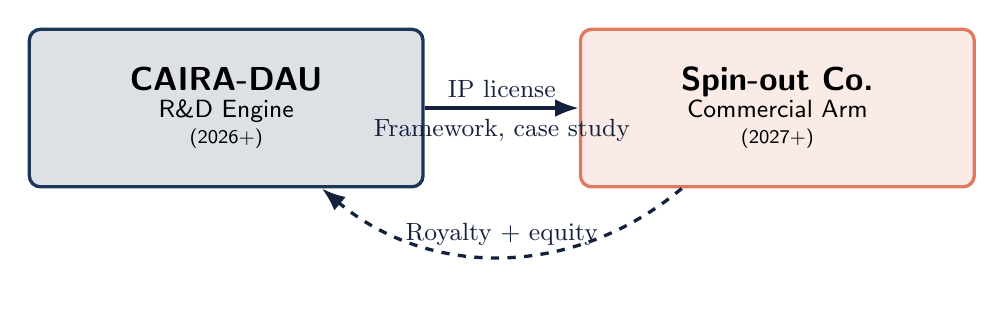
\begin{tikzpicture}[font=\sffamily\footnotesize]
  \node[rectangle, draw=caira, very thick, rounded corners=4pt, fill=caira!15,
        minimum width=5cm, minimum height=2cm, align=center] (c) at (0,0)
        {\textbf{\large CAIRA-DAU}\\\small R\&D Engine\\\scriptsize (2026+)};
  \node[rectangle, draw=spinout, very thick, rounded corners=4pt, fill=spinout!15,
        minimum width=5cm, minimum height=2cm, align=center] (s) at (7,0)
        {\textbf{\large Spin-out Co.}\\\small Commercial Arm\\\scriptsize (2027+)};
  \draw[-{Latex[length=3mm]}, very thick, ink] (c) -- node[above, font=\small]{IP license} node[below, font=\small]{Framework, case study} (s);
  \draw[-{Latex[length=3mm]}, very thick, ink, dashed] (s) to[bend left=40] node[above, font=\small]{Royalty + equity} (c);
\end{tikzpicture}

\vspace{3em}
{\large\color{ink}\sffamily
TS. Đỗ Phúc Hảo — Giám đốc CAIRA-DAU\\
Trường Đại học Kiến trúc Đà Nẵng
}\\[1em]
{\sffamily\color{mid} Đà Nẵng, tháng 4 năm 2026}
\end{center}
\vfill
\begin{center}
{\footnotesize\itshape\color{mid}
Tài liệu này thay thế các đề án ``startup độc lập'' trước đó. CAIRA-DAU là nền\\
tảng chính thức để xây dựng framework agentic AI, và Spin-out 2027 là bước\\
thương mại hoá sau khi có bằng chứng vận hành thật tại DAU.}
\end{center}
\clearpage

\tableofcontents
\clearpage

% =============================================================
% EXECUTIVE SUMMARY
% =============================================================
\section*{Tóm tắt điều hành}
\addcontentsline{toc}{section}{Tóm tắt điều hành}

\begin{keybox}[title=Tái định vị chiến lược trong 1 câu]
\textbf{Mục tiêu chính năm 2026 là xây dựng CAIRA-DAU thành một R\&D center
thành công, đạt KPI chính thức và triển khai 2 use case agentic AI thật tại
DAU. Spin-out 2027 là \textit{option upside}, không phải \textit{cam kết bắt
buộc}} --- chỉ được kích hoạt khi có bằng chứng thị trường bên ngoài thật sự
(discovery + LoI + market pull).
\end{keybox}

\textbf{Đây là một ``asymmetric bet'' với floor rất cao.} Kể cả kịch bản xấu
nhất (chỉ DAU dùng, không spin-out), đầu ra vẫn là:

\begin{itemize}
\item CAIRA đạt KPI 2026-2027 → thành công về mặt học thuật, hành chính.
\item 2 hệ thống agentic chạy thật tại DAU → giá trị thực cho Nhà trường.
\item 1-2 paper công bố + thương hiệu nghiên cứu → career advancement cho Hảo.
\item Phú có 12-18 tháng exp production AI → giá trị thị trường lao động tăng 2-3$\times$.
\item 0 VND mất từ tiền cá nhân của founders (CAIRA được DAU tài trợ).
\end{itemize}

\textbf{Nói cách khác:} mô hình này không phải ``thắng thị trường thì sống,
thua thì chết''. Mô hình này là ``thắng thị trường thì scale sang công ty,
không thắng vẫn có R\&D center thành công'' --- không có kịch bản failure
catastrophe.

\textbf{Lý do chọn mô hình này (thay vì mở công ty độc lập ngay 2026):}

\begin{enumerate}
\item \textbf{CAIRA đã có mandate chính thức} phù hợp 100\% với tầm nhìn agentic AI cho giáo dục: Đổi mới sáng tạo — R\&D — Ứng dụng/Chuyển giao.
\item \textbf{DAU trở thành design partner \#0} một cách tự nhiên, giải được câu hỏi khó nhất ``vì sao không làm cho trường mình''.
\item \textbf{Giảm rủi ro cá nhân 2026} — Hảo vẫn có lương, có văn phòng, có team trong vỏ bọc pháp nhân; Phú tiếp tục vai trò PM hiện có; Hoàng làm advisor có thù lao.
\item \textbf{IP rõ ràng} — framework được xây trong CAIRA với cơ chế sở hữu minh bạch, có thể license ra spin-out vào 2027 \textit{nếu} đủ điều kiện.
\item \textbf{Đồng thời đạt KPI CAIRA chính thức} — 2 sản phẩm số, 1 hệ thống triển khai tại DAU, 3-5 công bố, 2 MoU — đây \textit{đồng thời} là vật liệu cho spin-out nếu quyết định spin-out, và là thành tựu CAIRA độc lập nếu không.
\item \textbf{Quyết định spin-out dựa trên dữ liệu, không dựa trên hy vọng.} Tại Gate 2 (cuối Q1/2027), 3 người review dữ liệu validation (Chương 8) và quyết định go/no-go.
\end{enumerate}

\textbf{Điểm cần chấp nhận:}
\begin{itemize}
\item Hoàng phải chờ 12 tháng để \textit{có thể} thành co-founder. Spin-out có thể không xảy ra --- cần có ``exit path'' cho Hoàng nếu không spin-out (xem Chương 15).
\item IP sẽ thuộc DAU và license cho spin-out (\textit{nếu} spin-out), không phải full founder-owned.
\item Spin-out 2027 (\textit{nếu} được kích hoạt) cần phê duyệt chính thức của Hiệu trưởng DAU.
\item 3 người phải chấp nhận nguyên tắc ``thành công không đồng nghĩa với spin-out''.
\end{itemize}

\textbf{Bố cục tài liệu:}
\begin{itemize}
\item \textcolor{caira}{\textbf{Phần I--II (màu xanh navy)}} — CAIRA vận hành 2026.
\item \textcolor{spinout}{\textbf{Phần III--IV (màu cam)}} — Chuẩn bị và thực thi spin-out 2027.
\item Phần V — Vai trò con người và cam kết.
\item Phần VI — Rủi ro và quản trị.
\end{itemize}

\clearpage

% =============================================================
% PART I — KHUNG CHIẾN LƯỢC
% =============================================================
\begin{center}
\vspace*{0.5em}
{\sffamily\bfseries\Huge\color{caira} Phần I}\\[0.5em]
{\sffamily\LARGE\color{mid} Khung chiến lược}\\[0.5em]
{\color{caira}\rule{6cm}{0.4pt}}
\end{center}
\vspace{1em}

% =============================================================
\section{Tái định vị: CAIRA là mục tiêu chính, Spin-out là option}

\subsection{Nguyên tắc optionality --- đọc trước mọi thứ khác}

Tài liệu này dễ bị đọc sai nếu không hiểu nguyên tắc nền tảng này.

\begin{keybox}[title=Hai mức thành công]
\textbf{Mức 1 (bắt buộc, là mục tiêu chính):} CAIRA-DAU hoạt động thành công, đạt
KPI 2026-2027 chính thức, triển khai 2 use case thật tại DAU, xây được framework
tái sử dụng, có paper \& thương hiệu nghiên cứu.

\textbf{Mức 2 (option upside, không bắt buộc):} Spin-out thành công ty thương mại
với DAU là cổ đông sáng lập --- \textit{chỉ khi} có bằng chứng market pull bên
ngoài DAU (3+ LoI, 2+ workshop attendee quay lại, khách trả phí ký được).
\end{keybox}

\subsubsection*{Vì sao phải nhấn mạnh ``optionality''?}

Nhiều founder xuất thân academic rơi vào bẫy ``đã quyết là phải làm'' --- một
khi bắt đầu nói về ``công ty'', họ cảm thấy buộc phải thành lập công ty, kể cả
khi dữ liệu nói không. Đây là \textit{sunk cost fallacy} áp dụng cho commitment
chưa làm ra.

Với CAIRA-first, Hảo được giải thoát khỏi áp lực đó. Anh chỉ cần build CAIRA
tốt. Spin-out là quyết định độc lập, dựa trên dữ liệu Q1/2027, \textit{không} dựa
trên cam kết tinh thần đã làm từ 2026.

\subsubsection*{3 kịch bản outcome đều là ``thành công''}

\begin{tabularx}{\linewidth}{@{}p{2.5cm} p{3cm} X@{}}
\toprule
\textbf{Kịch bản} & \textbf{Xác suất est.} & \textbf{Outcome} \\
\midrule
\textbf{Best case} & 30-40\% & CAIRA + Spin-out hoạt động, 5-10 khách ngoài DAU năm 2027. Career \& tài chính big win. \\
\textbf{Base case} & 40-50\% & CAIRA thành công, nhưng không đủ market pull để spin-out. Hoàng rời với retainer đã nhận, Phú tiếp tục CAIRA hoặc chuyển sang cơ hội khác. Hảo có Director position mạnh. \\
\textbf{Worst case} & 10-20\% & Admissions Agent không đạt KPI tại DAU, cần rework. Kéo dài timeline. Không spin-out. Nhưng CAIRA vẫn đạt một số KPI khác (paper, events, hạ tầng). \\
\bottomrule
\end{tabularx}

\textbf{Tất cả 3 kịch bản đều không có ``phá sản cá nhân''} --- đây là đặc điểm
định nghĩa asymmetric bet với floor cao.

\subsection{Bức tranh 24 tháng}

\begin{center}
\begin{tikzpicture}[font=\sffamily, scale=1]
  % Timeline
  \draw[ink!60, very thick] (0,0) -- (16,0);
  \foreach \x/\m in {0/04-2026, 4/10-2026, 8/04-2027, 12/10-2027, 16/04-2028} {
    \draw[ink!60, thick] (\x,0.15) -- (\x,-0.15);
    \node[below=1mm, font=\footnotesize] at (\x,-0.15) {\m};
  }

  % CAIRA phase
  \node[rectangle, draw=caira, fill=caira!20, rounded corners=3pt,
        minimum width=9cm, minimum height=11mm, align=center, font=\footnotesize\sffamily] at (4,1.3)
        {\textbf{Giai đoạn 1 — CAIRA R\&D Phase}\\\scriptsize Xây framework + 2 use case DAU, thought leadership, discovery ngoài};

  % Spin-out phase
  \node[rectangle, draw=spinout, fill=spinout!25, rounded corners=3pt,
        minimum width=8cm, minimum height=11mm, align=center, font=\footnotesize\sffamily] at (12,1.3)
        {\textbf{Giai đoạn 2 — Spin-out Commercial Phase}\\\scriptsize Công ty thành lập, bán ra ngoài DAU};

  % Gates
  \foreach \x/\label in {4/G1, 8/G2, 12/G3, 16/G4} {
    \node[diamond, draw=warn, fill=warn!30, minimum size=6mm, font=\tiny\sffamily\bfseries] at (\x,2.7) {\label};
  }

  \node[font=\tiny\sffamily, align=center, text width=2.5cm] at (4,3.5) {Framework v0.5\\+ Admissions Agent DAU};
  \node[font=\tiny\sffamily, align=center, text width=2.5cm] at (8,3.5) {Spin-out\\go/no-go};
  \node[font=\tiny\sffamily, align=center, text width=2.5cm] at (12,3.5) {3 khách ngoài DAU};
  \node[font=\tiny\sffamily, align=center, text width=2.5cm] at (16,3.5) {ARR ổn định};

  % Milestones on timeline
  \node[font=\tiny\sffamily, ink, align=center, text width=2cm] at (0,-0.8) {CAIRA\\khởi động};
  \node[font=\tiny\sffamily, ink, align=center, text width=2cm] at (8,-0.8) {Spin-out\\thành lập};
\end{tikzpicture}
\end{center}

\subsection{3 nguyên tắc định vị}

\subsubsection*{Nguyên tắc 1 — CAIRA và Spin-out là 2 pháp nhân, 1 lộ trình}

CAIRA là đơn vị cấp trường, trực thuộc DAU, hoạt động theo quy chế công lập. Spin-out
là công ty TNHH thương mại. Hai pháp nhân, nhưng **một lộ trình chiến lược**: R\&D
chất lượng cao ở CAIRA → commercialize ở Spin-out → royalty về DAU/CAIRA → tái
đầu tư vào R\&D.

\subsubsection*{Nguyên tắc 2 — Framework thuộc DAU, Spin-out được license}

IP của framework được xây bằng nguồn lực CAIRA (ngân sách Nhà trường, cloud
được tài trợ, thời gian biên chế của Hảo, vai trò PM của Phú). Do đó \textbf{DAU
là chủ sở hữu IP}. Spin-out mua/license lại theo cơ chế chính thức: \textit{exclusive
license ngoài giáo dục đại học thuộc DAU}, kèm royalty và equity cho DAU.

Đây không phải rào cản — đây là \textbf{cơ chế chuẩn} cho mọi university spin-out:
MIT, Stanford, Ben-Gurion, Tel Aviv, KAIST đều dùng mô hình này.

\subsubsection*{Nguyên tắc 3 — Mỗi hoạt động 2026 phải đạt \textit{đồng thời} 3 mục tiêu}

\begin{itemize}
\item Đạt KPI CAIRA 2026-2027 chính thức (trách nhiệm với Nhà trường).
\item Xây IP có giá trị thương mại cho spin-out 2027.
\item Tạo bằng chứng vận hành \& case study cho sales motion 2027.
\end{itemize}

\textbf{Nếu một hoạt động không đạt được cả 3, không làm.} Đây là bộ lọc ưu tiên
xuyên suốt năm 1.

\clearpage

% =============================================================
\section{Mapping mandate CAIRA ↔ Framework agentic}

\subsection{3 trụ cột CAIRA ↔ 6 khối framework}

\begin{tabularx}{\linewidth}{@{}p{3.5cm} X@{}}
\toprule
\textbf{Trụ cột CAIRA} & \textbf{Framework agentic tương ứng} \\
\midrule
\textbf{Đổi mới sáng tạo} & Pattern library (5 pattern), hackathon kết nối sinh viên,
innovation challenge với sinh viên DAU để tìm use case thứ 3-5. \\
\textbf{Nghiên cứu phát triển} & 6 khối framework (Knowledge, Workflow, Tools, Reasoning,
Evals, Governance). Mỗi khối là một sub-project với paper khả dĩ. \\
\textbf{Ứng dụng \& Chuyển giao} & Triển khai 2 use case tại DAU: Admissions Agent
+ Internal Knowledge Agent. Đào tạo ngắn hạn về agentic AI cho giảng viên/cán bộ. \\
\bottomrule
\end{tabularx}

\subsection{Mapping 4 hướng ưu tiên CAIRA ↔ roadmap sản phẩm}

CAIRA đề án liệt kê 4 cụm ưu tiên (mục 8):

\begin{enumerate}
\item \textbf{Công nghệ cho giáo dục đại học} → Admissions Agent, Student Services
Agent (2026-2027).
\item \textbf{Công nghệ cho quản trị đại học} → Internal Knowledge Agent, SOP
Agent (2026-2027).
\item \textbf{Công nghệ cho kiến trúc-xây dựng} → Dùng riêng của DAU, không
commercial hoá (hoặc để sau 2028).
\item \textbf{Công nghệ liên ngành (kinh tế, du lịch, ngôn ngữ)} → Cho năm 2
spin-out (Service Operations Agent).
\end{enumerate}

\textbf{Chiến lược ưu tiên:} Hướng 1 + 2 tập trung 90\% nguồn lực 2026. Hướng 3
giữ lại như ``signature'' của DAU (khác biệt đặc thù). Hướng 4 chỉ nghiên cứu
sơ bộ, chờ spin-out 2027.

\subsection{KPI CAIRA 2026-2027 ↔ Milestones spin-out}

Đây là mapping quan trọng nhất --- mỗi KPI CAIRA chính thức \textit{đồng thời} là
milestone spin-out:

\begin{tabularx}{\linewidth}{@{}p{0.5cm} p{5.5cm} X@{}}
\toprule
\textbf{\#} & \textbf{KPI CAIRA 2026-2027} & \textbf{Ý nghĩa cho spin-out} \\
\midrule
1 & 2 nhóm NC ưu tiên hoạt động thường xuyên & Core engineering team + Domain research team \\
2 & 3-5 bài báo học thuật phản biện & Academic credibility cho thương hiệu spin-out \\
3 & 2 sản phẩm số/module phát triển thử nghiệm & Admissions Agent + Internal Knowledge Agent \\
4 & 1 hệ thống triển khai thực tế tại DAU & Case study \#1 cho sales motion 2027 \\
5 & 4 sự kiện/seminar/workshop & Thought leadership pipeline + tuyển dụng RA \\
6 & 10-15 sinh viên lab, RA, cộng tác viên & Hiring pipeline cho spin-out 2027 \\
7 & 2 MoU đối tác doanh nghiệp & 2 LoI với trường/DN cho giai đoạn đầu spin-out \\
8 & 1 khoá đào tạo ngắn hạn có thu phí & Revenue stream phụ + thương hiệu nhà cung cấp \\
9 & 1-2 đề tài/dự án R\&D được triển khai & Funding non-dilutive cho R\&D \\
10 & Tỷ lệ tự tạo < 10\% & Baseline trước khi spin-out tách ra \\
\bottomrule
\end{tabularx}

\textbf{Hàm ý:} Đạt 7/10 KPI CAIRA 2026-2027 đồng nghĩa với sẵn sàng spin-out.
Không đạt $\geq$ 6 KPI → chưa sẵn sàng, kéo dài CAIRA phase thêm 6-12 tháng.

\clearpage

% =============================================================
\section{Lộ trình 24 tháng}

\subsection{Giai đoạn 1 — CAIRA R\&D Phase (04-2026 đến 03-2027)}

\textbf{Sứ mệnh giai đoạn:} Chứng minh mô hình agentic AI hoạt động thật tại DAU, xây framework v1 có thể license được.

\begin{tabularx}{\linewidth}{@{}p{1.8cm} X@{}}
\toprule
\textbf{Quý} & \textbf{Trọng tâm \& deliverables} \\
\midrule
\textbf{Q2/2026} & \textit{Khởi động CAIRA.} Hoàn thiện quy chế, tuyển 3-5 RA, mua cloud/GPU, lập GitHub nội bộ, viết kế hoạch R\&D chi tiết. Hảo viết discovery doc cho Admissions use case tại DAU. \\
\textbf{Q3/2026} & \textit{Build skeleton framework + Admissions v0.} Phú dẫn build Knowledge + Workflow + Reasoning cơ bản. Ingest tài liệu tuyển sinh DAU. Demo prototype nội bộ. \\
\textbf{Q4/2026} & \textit{Pilot Admissions Agent tại DAU.} Shadow mode 4 tuần, HITL 4 tuần. Đo KPI thật trên dữ liệu thật. Submit 1 paper ACL/EMNLP/ICCL. Viết case study nội bộ. \\
\textbf{Q1/2027} & \textit{Admissions Agent autonomous + Internal Knowledge v0.} Go-live full. Bắt đầu build use case 2 (Internal Knowledge). Workshop CAIRA lần đầu mời 20-30 trường đến. \\
\bottomrule
\end{tabularx}

\subsection{Giai đoạn 2 — Spin-out Commercial Phase (04-2027 đến 03-2028)}

\textbf{Sứ mệnh giai đoạn:} Thương mại hoá framework ra ngoài DAU, xây nền tảng kinh tế độc lập.

\begin{tabularx}{\linewidth}{@{}p{1.8cm} X@{}}
\toprule
\textbf{Quý} & \textbf{Trọng tâm} \\
\midrule
\textbf{Q2/2027} & \textit{Thành lập spin-out.} Ký pháp lý: DAU là cổ đông sáng lập (IP license). Hảo, Phú, Hoàng ký founder agreement. Thuê văn phòng nhỏ riêng. \\
\textbf{Q3/2027} & \textit{Khách trả phí đầu tiên.} Chuyển 2-3 trường từ pipeline 2026 thành pilot trả phí. Nhịp delivery 8-10 tuần/khách. \\
\textbf{Q4/2027} & \textit{3-5 khách ngoài DAU.} Có doanh thu lặp lại. Framework v2 từ học được qua 3 khách. \\
\textbf{Q1/2028} & \textit{Packaging \& standardization.} Chuẩn hoá solution \#1. Bắt đầu nói chuyện angel / strategic investor nếu cần thêm vốn. \\
\bottomrule
\end{tabularx}

\subsection{4 decision gates}

\begin{tabularx}{\linewidth}{@{}p{1.2cm} p{2.5cm} X X@{}}
\toprule
\textbf{Gate} & \textbf{Thời điểm} & \textbf{Điều kiện pass} & \textbf{Nếu fail} \\
\midrule
G1 & 10-2026 & Framework v0.5 chạy được, Admissions Agent pilot bắt đầu tại DAU & Gia hạn Q4 thêm 1 quý, không bắt đầu use case 2 \\
G2 & 04-2027 & Admissions Agent live tại DAU đủ 3 tháng với KPI đạt; 3 trường ngoài đã sign LoI pilot & Hoãn spin-out 6 tháng, tiếp tục phase 1 \\
G3 & 10-2027 & Spin-out có $\geq$ 3 khách trả phí; framework v2 & Không thuê văn phòng lớn hơn; không tuyển thêm \\
G4 & 04-2028 & ARR $\geq$ 3 tỷ, NDR $\geq$ 100\% & Lùi kế hoạch mở rộng ĐNA \\
\bottomrule
\end{tabularx}

\clearpage

% =============================================================
% PART II — CAIRA VẬN HÀNH 2026
% =============================================================
\begin{center}
\vspace*{0.5em}
{\sffamily\bfseries\Huge\color{caira} Phần II}\\[0.5em]
{\sffamily\LARGE\color{mid} CAIRA vận hành 2026}\\[0.5em]
{\color{caira}\rule{6cm}{0.4pt}}
\end{center}
\vspace{1em}

% =============================================================
\section{Tổ chức \& Vai trò 3 người trong CAIRA 2026}

\subsection{Sơ đồ tổ chức CAIRA 2026}

\begin{center}
\begin{tikzpicture}[font=\sffamily\footnotesize,
  box/.style={draw=caira, rounded corners=3pt, minimum width=3cm, minimum height=1cm, align=center, inner sep=3pt}
]
  \node[box, fill=caira!30] (gd) at (0,4) {\textbf{Giám đốc CAIRA}\\\small TS. Đỗ Phúc Hảo};

  \node[box, fill=caira!15] (rd) at (-5,2) {\textbf{Nhóm R\&D / Kỹ thuật}\\\small PM \& Engineer trưởng\\\small Lê Hữu Phú};
  \node[box, fill=caira!15] (app) at (0,2) {\textbf{Ứng dụng \& Chuyển giao}\\\small Advisor thương mại\\\small Nguyễn Ngọc Hoàng (PT)};
  \node[box, fill=caira!15] (oi) at (5,2) {\textbf{Đổi mới sáng tạo}\\\small Events \& Network\\\small \textit{TBD} (kiêm nhiệm)};

  \node[box, fill=mid!20, minimum width=2.2cm] (e1) at (-6.5,0) {Engineer \#1\\\scriptsize từ M6};
  \node[box, fill=mid!20, minimum width=2.2cm] (e2) at (-4,0) {2 RA SV\\\scriptsize liên tục};
  \node[box, fill=mid!20, minimum width=2.2cm] (e3) at (-1,0) {Evals/QA\\\scriptsize part-time};

  \draw[-{Latex[length=2mm]}, ink] (gd) -- (rd);
  \draw[-{Latex[length=2mm]}, ink] (gd) -- (app);
  \draw[-{Latex[length=2mm]}, ink] (gd) -- (oi);
  \draw[-{Latex[length=2mm]}, ink] (rd) -- (e1);
  \draw[-{Latex[length=2mm]}, ink] (rd) -- (e2);
  \draw[-{Latex[length=2mm]}, ink] (rd) -- (e3);
\end{tikzpicture}
\end{center}

\subsection{Hảo — Giám đốc CAIRA}

\textbf{Vai trò chính thức:} Giám đốc Trung tâm CAIRA-DAU (đã được bổ nhiệm 17/4/2026).

\textbf{Thời lượng cam kết:} Toàn thời gian CAIRA + giảng dạy giảm xuống tối thiểu cần thiết (4-6 tiết/tuần). **Không nhận thêm dự án tư vấn/nghiên cứu ngoài không phục vụ CAIRA.**

\textbf{Trách nhiệm năm 2026:}
\begin{enumerate}
\item Lãnh đạo CAIRA đạt KPI 2026-2027 chính thức.
\item Quan hệ với Hiệu trưởng/Ban Giám hiệu DAU; xin phê duyệt nguyên tắc spin-out trong Q3/2026.
\item Discovery workshop với phòng Tuyển sinh DAU; mở rộng sang phòng Công tác sinh viên, Đào tạo.
\item Academic output: 1-2 paper, 4 seminar/workshop, 1 talk chính thức/quý.
\item External network: 10-15 trường quen qua hội thảo/thư viện quan hệ; KHÔNG sell, chỉ trao đổi học thuật.
\item Chuẩn bị cấu trúc spin-out (pháp lý, IP, equity) Q4/2026.
\end{enumerate}

\textbf{Không làm:} viết code production (chỉ prototype được), quản lý timeline delivery, trực tiếp tìm khách bên ngoài (Hoàng làm), nhận lời mời tư vấn/giảng dạy ngoài DAU.

\subsection{Phú — PM \& Engineering Lead (chức danh CAIRA)}

\textbf{Vai trò chính thức trong CAIRA:} \textit{Trưởng nhóm R\&D / Kỹ thuật trưởng} (hợp đồng lao động CAIRA, có thể kiêm vai PM dự án trường hiện tại nếu khối lượng cho phép).

\textbf{Lợi thế cấu trúc:} Phú đã đang làm PM cho dự án tại trường → về mặt hành chính, bổ sung vai trò CAIRA không khó. Phú là cựu sinh viên + học trò Hảo → tin tưởng lẫn nhau sẵn có, không cần giai đoạn ``quen việc chung''.

\textbf{Cam kết:}
\begin{itemize}
\item Thời lượng: tối thiểu 80\% CAIRA, tối đa 20\% dự án trường hiện tại.
\item Hợp đồng: nhân sự CAIRA theo dự án (mục 9 Đề án CAIRA) — không biên chế, có lương.
\item Thù lao: ngang hoặc cao hơn thị trường kỹ sư AI junior+ tại Đà Nẵng (15--25 triệu/tháng tuỳ cơ chế CAIRA).
\item Cam kết đi cùng: tối thiểu 24 tháng (2026-2027), với kỳ vọng trở thành co-founder spin-out 2027.
\end{itemize}

\textbf{Trách nhiệm 2026:}
\begin{enumerate}
\item Xây framework 6 khối (v0 → v1.0 trong 9-12 tháng).
\item Dẫn build 2 use case tại DAU (Admissions + Internal Knowledge).
\item Tuyển và mentor 1-2 engineer junior + 2-3 RA sinh viên.
\item Chuẩn hoá quy trình delivery (documentation, evals, CI/CD).
\item Chuẩn bị architecture để transfer sang spin-out 2027.
\end{enumerate}

\textbf{Pre-commitment cho 2027:} Phú sẽ là \textbf{CTO \& co-founder} của spin-out với equity 20-25\% (chi tiết ở chương 12). Điều này được ghi trong LoI (chương 14).

\subsection{Hoàng — Advisor Thương mại \& Chuyển giao (part-time)}

\textbf{Đây là vai trò khó nhất để cấu trúc} — Hoàng là connection bên ngoài, chưa trong DAU, và đang có công việc riêng.

\textbf{Đề xuất vai trò:} \textit{Cố vấn Trưởng nhóm Ứng dụng \& Chuyển giao} (part-time, hợp đồng dịch vụ chuyên môn, không biên chế).

\textbf{Cấu trúc cam kết:}
\begin{itemize}
\item Thời lượng: 20-30\% (tuần $\sim$ 8-12h).
\item Hợp đồng: \textbf{Dịch vụ chuyên môn} (không phải nhân sự CAIRA). CAIRA mục 11 cho phép ``dịch vụ chuyên môn có thu phí''. Có thể ngược lại: Hoàng cung cấp dịch vụ tư vấn cho CAIRA.
\item Thù lao: per-meeting hoặc monthly retainer (5-10 triệu/tháng), tuỳ đàm phán.
\item Giữ công việc hiện tại: \textbf{có thể}, miễn không xung đột lợi ích.
\end{itemize}

\textbf{Trách nhiệm 2026:}
\begin{enumerate}
\item Tư vấn CAIRA về cách package sản phẩm để chuyển giao (khoá đào tạo, tư vấn, sản phẩm số).
\item Dẫn 10-15 discovery call với trường/doanh nghiệp (KHÔNG ký hợp đồng thương mại, chỉ LoI hoặc MoU). Đây là pipeline cho spin-out 2027.
\item Giúp CAIRA đạt KPI \#7 (2 MoU đối tác doanh nghiệp).
\item Tham gia 1 sự kiện CAIRA lớn (thuyết trình về thương mại hoá).
\end{enumerate}

\textbf{Pre-commitment cho 2027:} Hoàng sẽ là \textbf{CEO \& co-founder} của spin-out với equity 20-25\%. Điều này được ghi trong LoI.

\begin{warnbox}[title=Vấn đề phải đối thoại thẳng với Hoàng]
Hoàng kỳ vọng làm CEO \textbf{ngay}. Mô hình CAIRA-first yêu cầu Hoàng \textit{chờ 12
tháng} làm advisor trước khi thành CEO. Cần cuộc đối thoại 1-1 giữa Hảo và Hoàng
để:
\begin{itemize}
\item Trình bày rõ lý do chiến lược (lợi thế pháp lý, IP, DAU là design partner)
\item Đề xuất compensation hợp lý cho 12 tháng chờ (retainer + equity lock-in)
\item Nếu Hoàng không đồng ý → chương 14 có kịch bản backup
\end{itemize}
\end{warnbox}

\clearpage

% =============================================================
\section{Kế hoạch 4 quý năm 2026}

\subsection{Q2/2026 (tháng 4-6) — Khởi động CAIRA}

\subsubsection*{Mục tiêu quý}

\begin{itemize}
\item Hoàn thiện tổ chức \& quy chế CAIRA chính thức đi vào hoạt động.
\item Tuyển đủ nhân sự cốt lõi: 2-3 RA sinh viên + 1 engineer junior part-time.
\item Mua cloud + GPU. Thiết lập repo, CI/CD, dev environment.
\item Hoàn thành discovery với phòng Tuyển sinh DAU.
\item Đồng thuận 3 người (Hảo, Phú, Hoàng) về LoI và roadmap.
\end{itemize}

\subsubsection*{Deliverables cụ thể}

\begin{tabularx}{\linewidth}{@{}p{3.5cm} X@{}}
\toprule
\textbf{Deliverable} & \textbf{Owner \& deadline} \\
\midrule
Quy chế CAIRA hoàn thiện & Hảo + Phòng Tổ chức, tuần 2 \\
Founder LoI 3 bên ký & Hảo, tuần 3 \\
Repo GitHub + infra sẵn sàng & Phú, tuần 4 \\
Tuyển 3 RA sinh viên khoa CNTT & Phú, cuối tháng 5 \\
Discovery report Tuyển sinh DAU & Hảo, cuối tháng 5 \\
R\&D plan chi tiết Q3-Q4 & Hảo + Phú, cuối tháng 6 \\
First seminar nội bộ (kickoff event) & Hảo, cuối tháng 6 \\
\bottomrule
\end{tabularx}

\subsection{Q3/2026 (tháng 7-9) — Build skeleton framework + Admissions v0}

\subsubsection*{Mục tiêu quý}

\begin{itemize}
\item Framework 6 khối v0 có thể chạy end-to-end với use case đơn giản.
\item Admissions Agent v0 chạy được trên dữ liệu DAU (chưa deploy production).
\item Viết first paper (hoặc working paper).
\item Tổ chức hackathon/workshop nhỏ mời sinh viên các khoa khác.
\end{itemize}

\subsubsection*{Deliverables cụ thể}

\begin{tabularx}{\linewidth}{@{}p{4cm} X@{}}
\toprule
\textbf{Deliverable} & \textbf{Ghi chú} \\
\midrule
Knowledge layer + Workflow layer v0 & Ingestion PDF tuyển sinh DAU; state machine đơn giản \\
Reasoning layer với 1 pattern (Q\&A) & Claude + pgvector + Vietnamese embedding \\
Evals v0 với 30 golden case & Lấy từ log Zalo DAU 2025 \\
Admissions Agent v0 demo & Chạy offline trên dữ liệu test \\
Working paper về approach & Để submit Q4 \\
Hackathon CAIRA ``AI cho DAU'' & 20-30 sinh viên, 48h \\
\bottomrule
\end{tabularx}

\subsection{Q4/2026 (tháng 10-12) — Pilot Admissions Agent tại DAU}

\subsubsection*{Mục tiêu quý}

\begin{itemize}
\item Admissions Agent chạy pilot thật tại phòng Tuyển sinh DAU.
\item Đạt KPI baseline: auto-resolve $\geq$ 40\% (cao hơn target quản lý, thấp hơn target dài hạn 60\%).
\item Submit paper chính thức.
\item Bắt đầu external engagement (workshop mời 2-3 trường bạn).
\item Chuẩn bị pháp lý spin-out (working paper với Hiệu trưởng).
\end{itemize}

\subsubsection*{Deliverables}

\begin{tabularx}{\linewidth}{@{}p{4cm} X@{}}
\toprule
\textbf{Deliverable} & \textbf{Ghi chú} \\
\midrule
Admissions Agent pilot 2 tháng tại DAU & Shadow tháng 10, HITL tháng 11, auto 20\% tháng 12 \\
Monthly dashboard cho phòng Tuyển sinh & Transparency, chỉ số đo được \\
Case study internal v1 & Cho KPI \#4 CAIRA (hệ thống triển khai thực tế) \\
Paper submitted (ACL/EMNLP/VLSP) & Cho KPI \#2 \\
Workshop ``Agentic AI for University Operations'' & 30-50 người, DAU + 2-3 trường bạn \\
Initial discussion với Hiệu trưởng về spin-out & Hảo trực tiếp trình bày \\
\bottomrule
\end{tabularx}

\subsection{Q1/2027 (tháng 1-3) — Admissions autonomous + Internal Knowledge v0}

\subsubsection*{Mục tiêu quý}

\begin{itemize}
\item Admissions Agent go-live full autonomous.
\item Internal Knowledge Agent v0 (use case thứ 2).
\item Tổ chức CAIRA Conference lần đầu với 20-30 trường ngoài.
\item Hoàn tất đàm phán pháp lý spin-out (chờ ký).
\item Đạt KPI CAIRA 2026-2027 chính thức $\geq$ 70\%.
\end{itemize}

\begin{keybox}[title=Tại cuối Q1/2027 --- Gate 2: Go/No-go spin-out]
\textbf{Spin-out là quyết định riêng biệt tại Gate 2, dựa trên 3 loại bằng chứng:}

\textbf{(A) Bằng chứng sản phẩm:}
\begin{itemize}
\item Admissions Agent đạt KPI tại DAU (auto $\geq$ 50\%, CSAT $\geq$ 4.0, zero critical error)
\item Framework v1.0 stable, có thể deploy cho trường khác trong 6-8 tuần
\end{itemize}
\textbf{(B) Bằng chứng thị trường (validation Q3/2026--Q1/2027):}
\begin{itemize}
\item $\geq$ 10 discovery call với trường ngoài, có ghi chép chi tiết
\item $\geq$ 3 trường ngoài ký LoI quan tâm pilot trả phí
\item CAIRA Workshop (Q1/2027) có $\geq$ 3 trường follow-up với câu hỏi thương mại cụ thể
\end{itemize}
\textbf{(C) Bằng chứng cam kết con người \& tổ chức:}
\begin{itemize}
\item Phú \& Hoàng xác nhận sẵn sàng spin-out
\item Hảo sẵn sàng role dual-hat (CAIRA Director + Chairman)
\item DAU Hiệu trưởng/HĐT đồng ý nguyên tắc spin-out + equity model
\end{itemize}

\textbf{Quy tắc quyết định:} Phải đạt \textbf{ít nhất 2/3} ở MỖI nhóm A, B, C.
Không cho phép ``A đủ, B thiếu'' --- thiếu market validation thì không spin-out,
bất kể sản phẩm có tốt đến đâu.

\textbf{Nếu không đủ $\to$} kéo dài CAIRA phase 6 tháng, re-evaluate Q3/2027.
Hoặc chính thức quyết định ``không spin-out'' và tiếp tục CAIRA độc lập --- đây
là outcome hoàn toàn hợp lệ, không phải thất bại.
\end{keybox}

\clearpage

% =============================================================
\section{2 sản phẩm flagship năm 2026 tại DAU}

\subsection{Use case 1 — Admissions Agent (DAU phòng Tuyển sinh)}

Đây là product đầu tiên, cũng là product quan trọng nhất --- vì nó là
\textit{proof-of-concept} cho toàn bộ mô hình.

\textbf{Stakeholders DAU:}
\begin{itemize}
\item Sponsor: Phó Hiệu trưởng phụ trách Đào tạo / Tuyển sinh
\item Champion: Trưởng phòng Tuyển sinh
\item Users: 3-5 cán bộ tuyển sinh
\item Technical contact: Trưởng phòng CNTT / Trợ lý của Hảo
\end{itemize}

\textbf{Baseline \& target (đề xuất, chờ xác nhận sau discovery):}

\begin{tabularx}{\linewidth}{@{}p{4cm} X X@{}}
\toprule
\textbf{Metric} & \textbf{Baseline 2025} & \textbf{Target Q1/2027} \\
\midrule
Câu hỏi/tháng mùa cao điểm & TBD (est 3.000-5.000) & giữ volume \\
Thời gian phản hồi trung bình & TBD (est 3-6h) & $\leq$ 1 phút auto \\
\% câu tự xử lý & 0\% & $\geq$ 50\% \\
CSAT (nếu đo được) & --- & $\geq$ 4.0/5 \\
Cán bộ overtime (giờ/tuần) & TBD & giảm 40\%+ \\
\bottomrule
\end{tabularx}

\textbf{Dataset \& tài liệu (cần xin phép qua CAIRA → Phòng Tuyển sinh):}
\begin{itemize}
\item Tài liệu tuyển sinh 2024, 2025, 2026 (PDF, Word)
\item Học phí + quy chế từng ngành
\item Log Zalo OA Tuyển sinh 2024-2025 (anonymize)
\item FAQ nội bộ phòng Tuyển sinh
\item Brochure ngành (8 ngành)
\end{itemize}

\textbf{Timeline:}
\begin{itemize}
\item Tháng 5-6: Discovery, data agreement, data cleansing
\item Tháng 7-9: Build v0, internal demo
\item Tháng 10: Shadow mode
\item Tháng 11: HITL mode
\item Tháng 12: Auto 20\% traffic
\item Tháng 1/2027: Auto 100\% với escalation
\item Tháng 2/2027: Full production + case study paper
\end{itemize}

\subsection{Use case 2 — Internal Knowledge Agent}

Use case thứ 2, khởi động muộn hơn để Phú có bandwidth. Đây cũng là ``sản phẩm''
dùng chung nội bộ CAIRA/DAU nên có lợi ích kép: vừa là case study, vừa là tool
làm việc thật.

\textbf{Phạm vi:} Trợ lý trả lời câu hỏi về quy chế, quy định, SOP nội bộ DAU
cho cán bộ/giảng viên. Access-controlled theo vai trò.

\textbf{Timeline:}
\begin{itemize}
\item Q4/2026: Discovery (tuần 1 của Q4)
\item Q1/2027: Build v0
\item Q2/2027 (sau spin-out): Go-live
\end{itemize}

\subsection{Vì sao chọn 2 use case này, không phải khác}

\begin{itemize}
\item \textbf{Pain có thật, đo được:} Cả 2 đều giảm tải cán bộ, có KPI rõ.
\item \textbf{Dữ liệu sẵn có:} Tài liệu đều có, không cần xây dataset từ đầu.
\item \textbf{Risk thấp cho DAU:} Không ảnh hưởng sinh viên/phụ huynh mạnh nếu lỗi.
\item \textbf{Tương tự nhau về kỹ thuật:} Cả 2 đều Pattern 1 (Knowledge Q\&A), cho phép tái sử dụng framework $\geq$ 70\%.
\item \textbf{Dễ replicate sang trường khác:} Mọi trường đều có tuyển sinh + internal knowledge.
\end{itemize}

\clearpage

% =============================================================
\section{Framework development \& IP strategy}

\subsection{Framework là tài sản của DAU, không phải của cá nhân}

\textbf{Đây là điểm quan trọng phải nói thẳng:} Framework xây trong CAIRA, dùng
ngân sách và cơ sở vật chất của DAU, với thời gian biên chế của Hảo. Theo Luật
Khoa học \& Công nghệ và Luật Sở hữu trí tuệ Việt Nam, \textbf{DAU là chủ sở hữu
IP hợp pháp}.

Điều này \textbf{không phải trở ngại} cho spin-out --- ngược lại, đây là cơ chế
chuẩn cho mọi university spin-out quốc tế. Nhìn MIT, Stanford, KAIST, Weizmann:
mọi công ty spin-out đều license IP từ trường, và trả lại trường dưới dạng equity
+ royalty.

\subsection{Cơ chế IP đề xuất cho spin-out 2027}

\begin{tabularx}{\linewidth}{@{}p{3.5cm} X@{}}
\toprule
\textbf{Yếu tố} & \textbf{Đề xuất} \\
\midrule
Chủ sở hữu IP & DAU (cho framework core), \textit{joint ownership} (cho use case giáo dục specific như Admissions Agent) \\
Loại license cho spin-out & Exclusive license \textit{ngoài phạm vi DAU và các trường trong DAU ecosystem} \\
Royalty rate & 3-5\% doanh thu ngành giáo dục, 1-2\% ngành khác (đàm phán) \\
Equity của DAU trong spin-out & 10-15\% (nonvoting founding shareholder) \\
Thời hạn license & 20 năm, tự động gia hạn nếu spin-out đạt KPI royalty \\
Quyền kiểm soát chất lượng của DAU & DAU có seat trong Technical Advisory Board của spin-out \\
Quyền dùng nội bộ của DAU & Free in perpetuity cho DAU dùng nội bộ \\
Non-compete & Spin-out không được bán cho các đối thủ trực tiếp của DAU trong tuyển sinh (phạm vi Đà Nẵng) trong 3 năm \\
\bottomrule
\end{tabularx}

\subsection{Phân tách rõ IP của CAIRA vs của Spin-out}

\begin{center}
\begin{tikzpicture}[font=\sffamily\footnotesize,
  ip/.style={rectangle, draw=caira, rounded corners=2pt, fill=caira!10, minimum width=4.5cm, minimum height=0.8cm, align=center, inner sep=2pt},
  ipcom/.style={rectangle, draw=spinout, rounded corners=2pt, fill=spinout!15, minimum width=4.5cm, minimum height=0.8cm, align=center, inner sep=2pt}
]
  \node[font=\sffamily\bfseries\small, caira] at (-3.5,6) {IP thuộc DAU (qua CAIRA)};
  \node[ip] at (-3.5,5) {Framework 6 khối (core)};
  \node[ip] at (-3.5,4) {Patterns library};
  \node[ip] at (-3.5,3) {Evals methodology};
  \node[ip] at (-3.5,2) {Academic publications};
  \node[ip] at (-3.5,1) {Admissions Agent DAU (nội bộ)};

  \node[font=\sffamily\bfseries\small, spinout] at (3.5,6) {IP của Spin-out};
  \node[ipcom] at (3.5,5) {Customer-specific configs};
  \node[ipcom] at (3.5,4) {Admin dashboard thương mại};
  \node[ipcom] at (3.5,3) {Sales \& marketing materials};
  \node[ipcom] at (3.5,2) {Customer data (per customer agreement)};
  \node[ipcom] at (3.5,1) {Case studies ngoài DAU};

  \draw[-{Latex[length=2.5mm]}, very thick, ink] (-1,3) -- node[above, font=\tiny]{license} (1,3);
\end{tikzpicture}
\end{center}

\subsection{Xin phê duyệt nguyên tắc từ DAU — trong Q3/2026}

\textbf{Timeline đề xuất:}

\begin{enumerate}
\item \textbf{Tháng 7/2026:} Hảo chuẩn bị brief 3-5 trang gửi Hiệu trưởng về:
\begin{itemize}
\item Bối cảnh: CAIRA mandate có phần ``chuyển giao công nghệ''
\item Đề xuất: khi đạt KPI, spin-out với DAU là cổ đông sáng lập
\item Lợi ích cho DAU: equity + royalty + continued free use
\item Khung pháp lý tham khảo: Luật KH\&CN 2013, Nghị định 99/2014
\end{itemize}
\item \textbf{Tháng 8-9/2026:} Họp với Hiệu trưởng, Trưởng phòng Tổ chức-Hành chính, Trưởng phòng Kế toán-Tài chính, Trưởng phòng Quản lý Khoa học.
\item \textbf{Tháng 10/2026:} Có văn bản nguyên tắc (không cần MoU chi tiết). Chi tiết đàm phán khi thực sự ready spin-out (Q1/2027).
\end{enumerate}

\clearpage

% =============================================================
% PART III — CHUẨN BỊ SPIN-OUT
% =============================================================
\begin{center}
\vspace*{0.5em}
{\sffamily\bfseries\Huge\color{spinout} Phần III}\\[0.5em]
{\sffamily\LARGE\color{mid} Validation thị trường \& Chuẩn bị spin-out}\\[0.5em]
{\color{spinout}\rule{6cm}{0.4pt}}
\end{center}
\vspace{1em}

% =============================================================
\section{Validation thị trường --- cơ chế quyết định spin-out}

Chương này trình bày \textbf{cơ chế validation cụ thể} để quyết định Gate 2
(Q1/2027) có spin-out hay không. Đây là phần quan trọng nhất của
``optionality framework'' --- không có phần này, spin-out trở thành mơ mộng
chứ không phải quyết định có bằng chứng.

\subsection{3 loại bằng chứng validation cần thu thập 2026}

\subsubsection*{Bằng chứng A --- Product validation (nội bộ DAU)}

Đây là dễ nhất --- chỉ cần CAIRA chạy tốt là có.

\begin{tabularx}{\linewidth}{@{}p{4cm} p{3cm} X@{}}
\toprule
\textbf{Chỉ số} & \textbf{Target Q1/2027} & \textbf{Cách đo} \\
\midrule
Auto-resolve rate & $\geq$ 50\% & Production logs sau 3 tháng live \\
First-response time & $\leq$ 1 phút & P95 latency \\
CSAT score & $\geq$ 4.0/5 & Survey sau mỗi 10 conversation \\
Zero critical errors & 0 incident & Audit log \\
Framework reuse khi build use case 2 & $\geq$ 50\% & Code diff analysis \\
\bottomrule
\end{tabularx}

\subsubsection*{Bằng chứng B --- Market validation (ngoài DAU) — QUAN TRỌNG NHẤT}

Đây là bằng chứng then chốt mà nếu thiếu, tuyệt đối không spin-out.

\begin{tabularx}{\linewidth}{@{}p{4cm} p{3cm} X@{}}
\toprule
\textbf{Milestone} & \textbf{Thời điểm} & \textbf{Cụ thể} \\
\midrule
Discovery calls với trường ngoài & Q3-Q4/2026 & $\geq$ 10 cuộc, có ghi chép chi tiết, ít nhất 5 trường đồng ý follow-up. \\
Tình nguyện quan tâm pilot & Q4/2026 & $\geq$ 3 trường bày tỏ quan tâm cụ thể về pilot (chưa cần ký) \\
CAIRA Workshop attendance & Q1/2027 & $\geq$ 20 người đến từ $\geq$ 10 trường \\
Post-workshop follow-up & Q1/2027 & $\geq$ 3 trường follow-up trong 2 tuần với câu hỏi thương mại cụ thể (giá, timeline, scope) \\
\textbf{LoI ký ngoài DAU} & Q1/2027 & \textbf{$\geq$ 3 LoI --- hard threshold} \\
\bottomrule
\end{tabularx}

\textbf{Nguyên tắc:} Nếu không đạt $\geq$ 3 LoI ngoài DAU tại Gate 2, \textit{dù sản
phẩm tốt và các chỉ số khác tốt}, không spin-out. Thiếu market pull = spin-out
sẽ là outsourcing disguised.

\subsubsection*{Bằng chứng C --- Commitment validation (3 người + DAU)}

\begin{tabularx}{\linewidth}{@{}p{4cm} X@{}}
\toprule
\textbf{Điều kiện} & \textbf{Cách xác nhận} \\
\midrule
Phú sẵn sàng chuyển từ CAIRA sang spin-out (hoặc dual role) & Confirmation trực tiếp + kế hoạch vesting trong LoI \\
Hoàng sẵn sàng full-time CEO & Confirmation trực tiếp + plan quit current job \\
Hảo sẵn sàng dual-hat (CAIRA Director + Chairman) & Tự đánh giá + discussion với DAU \\
DAU đồng ý nguyên tắc spin-out + IP license + equity & Văn bản chính thức từ Hiệu trưởng \\
Có ít nhất 1 luật sư hoặc firm sẵn sàng handle pháp lý & Quote + availability confirmation \\
\bottomrule
\end{tabularx}

\subsection{Timeline validation}

\begin{center}
\begin{tikzpicture}[font=\sffamily\footnotesize,
  ms/.style={circle, draw=spinout, fill=spinout!25, minimum size=4mm, inner sep=0pt}
]
  \draw[ink!60, very thick] (0,0) -- (16,0);
  \foreach \x/\m in {0/04-2026, 3/07-2026, 6/10-2026, 9/01-2027, 12/03-2027, 15/04-2027} {
    \draw[ink!60, thick] (\x,0.15) -- (\x,-0.15);
    \node[below=1mm, font=\footnotesize] at (\x,-0.15) {\m};
  }

  \node[ms] at (4,0) {}; \node[above=2mm, font=\tiny, align=center, text width=2.5cm] at (4,0.3) {5 discovery call đầu};
  \node[ms] at (6,0) {}; \node[below=2mm, font=\tiny, align=center, text width=2.5cm] at (6,-0.9) {5 discovery call tiếp};
  \node[ms] at (8,0) {}; \node[above=2mm, font=\tiny, align=center, text width=2.5cm] at (8,0.3) {Workshop Q4};
  \node[ms] at (10,0) {}; \node[below=2mm, font=\tiny, align=center, text width=2.5cm] at (10,-0.9) {CAIRA Conference Q1/2027};
  \node[ms] at (11.5,0) {}; \node[above=2mm, font=\tiny, align=center, text width=2.5cm] at (11.5,0.3) {Đàm phán LoI};
  \node[diamond, draw=warn, fill=warn!30, minimum size=6mm, font=\tiny\sffamily\bfseries] at (13,0.8) {G2};
  \node[font=\tiny, align=center] at (13,1.7) {Go/No-go\\decision};
\end{tikzpicture}
\end{center}

\subsection{Điều gì nếu validation failed?}

\begin{tabularx}{\linewidth}{@{}p{4cm} X@{}}
\toprule
\textbf{Kịch bản failure} & \textbf{Phản ứng} \\
\midrule
Discovery calls không đủ 10 & Kéo dài 3 tháng, mở rộng network (hợp tác với hiệp hội giáo dục). Không spin-out Q2/2027. \\
$<$ 3 LoI ký được & Không spin-out. Hoặc điều chỉnh scope (chuyển sang đào tạo/tư vấn thay vì solution). \\
Workshop có ít attendee & Chuyển hướng: vẫn làm workshop nhưng trong DAU ecosystem thay vì cross-school. Điều chỉnh kế hoạch 2027. \\
DAU phản đối nguyên tắc spin-out & Không spin-out. CAIRA tiếp tục, commercialize nội bộ qua dịch vụ chuyên môn (mục 11 Đề án CAIRA). \\
1 hoặc 2 founder rút & Tuỳ ai rút và rút khi nào. Tham khảo Chương 14 điều 10, và Chương 15. \\
\bottomrule
\end{tabularx}

\textbf{Trong mọi kịch bản trên, CAIRA vẫn tiếp tục và vẫn có thể thành công
độc lập.} ``Không spin-out'' không phải thất bại --- đó chỉ là quyết định rằng
outcome tối ưu là giữ CAIRA.

\clearpage

% =============================================================
\section{External engagement 2026 — không sell, chỉ xây network}

\subsection{Nguyên tắc vàng: không sell trong 2026}

Trong năm 2026, \textbf{CAIRA không ký bất kỳ hợp đồng thương mại nào ngoài
DAU}. Lý do:

\begin{itemize}
\item CAIRA là đơn vị công lập, việc bán sản phẩm thương mại ra ngoài phải qua nhiều cơ chế phê duyệt.
\item Nếu CAIRA bán hợp đồng thương mại, IP dispute sẽ phức tạp khi spin-out.
\item Năm 2026 mục đích là \textit{xây brand}, \textit{discovery}, \textit{network}, không phải revenue.
\end{itemize}

Hoàng có thể đi meeting, có thể viết LoI, có thể ký MoU về nghiên cứu chung —
nhưng \textbf{không ký hợp đồng bán hàng}. Hợp đồng bán hàng đầu tiên là của spin-out, Q2-Q3/2027.

\subsection{3 hoạt động external chính trong 2026}

\subsubsection*{1. Thought leadership (Hảo chủ trì)}

\begin{itemize}
\item 2 bài báo khoa học submit/publish trong năm (ACL/EMNLP/VLSP cho technical; một bài ở tạp chí giáo dục Việt Nam cho domain).
\item 1 blog post/tháng trên LinkedIn cá nhân Hảo (tiếng Việt).
\item 1 talk/quý tại workshop/hội thảo giáo dục Việt Nam (ngành tuyển sinh, ngành CNTT giáo dục).
\item 1 podcast/interview/tháng cho báo/channel về AI \& giáo dục.
\end{itemize}

\subsubsection*{2. Network building (Hảo + Hoàng phối hợp)}

\textbf{Đối tượng target:}
\begin{itemize}
\item 20 trường ĐH tư thục/bán công ở Miền Trung + Miền Nam có $\geq$ 3.000 SV.
\item 5-7 trường ĐH công lập tầm trung có phòng hợp tác doanh nghiệp chủ động.
\item 3-5 hiệp hội/tổ chức ngành giáo dục (VEI, Hiệp hội Giáo dục Đại học).
\end{itemize}

\textbf{Cách tiếp cận:}
\begin{itemize}
\item \textbf{Hảo peer-to-peer:} ``Em đang triển khai nghiên cứu Agentic AI tại CAIRA DAU. Muốn xin 45 phút để chia sẻ kết quả ban đầu và học hỏi quy trình tuyển sinh của trường anh/chị.''
\item Đi cùng với tài liệu: working paper, slide CAIRA, demo Admissions Agent (sau Q3/2026).
\item Kết thúc meeting: đề xuất \textit{collaborative research} nếu trường có interest, không sell.
\end{itemize}

\textbf{KPI:} 10 discovery-style meeting trong Q3-Q4/2026 + 5 tiếp trong Q1/2027 = 15 trường trong pipeline.

\subsubsection*{3. CAIRA Conference (Q1/2027)}

Event lớn nhất năm CAIRA. Mục đích:
\begin{itemize}
\item Khẳng định vị thế CAIRA trong ngành giáo dục Việt Nam.
\item Tụ hội 20-30 trường để trao đổi về ứng dụng AI.
\item Giới thiệu Admissions Agent case study (đã chạy tại DAU).
\item \textbf{Không pitch sản phẩm}, chỉ chia sẻ thực tế và kết quả.
\end{itemize}

Sau event này → pipeline cho spin-out Q2/2027 có đủ lead cho 5-10 pilot.

\clearpage

% =============================================================
\section{Thought leadership \& Publications}

\subsection{2 paper chiến lược 2026}

\subsubsection*{Paper 1 — Technical}

\textbf{Tựa đề tạm:} ``An Agentic AI Framework for University Operations in
Low-Resource Vietnamese Context''

\textbf{Contribution:}
\begin{itemize}
\item Framework 6-khối cho agentic systems trong giáo dục VN.
\item Benchmark Vietnamese embedding + prompt strategies cho admissions Q\&A.
\item Ablation study: single-agent vs specialist vs supervisor pattern.
\item Evals methodology với 300+ case tiếng Việt.
\end{itemize}

\textbf{Target venue:} VLSP 2026 (ngắn), ACL 2027 Findings (dài), hoặc IEEE TALE
(giáo dục).

\textbf{Timeline:} Draft Q3/2026, submit Q4/2026, resubmit Q1/2027 nếu cần.

\subsubsection*{Paper 2 — Applied/Case study}

\textbf{Tựa đề tạm:} ``Deploying an AI Admissions Agent at a Vietnamese
University: Operational KPIs and Lessons Learned''

\textbf{Contribution:}
\begin{itemize}
\item Case study thực tế tại DAU (với baseline vs post-deploy metrics).
\item Framework for evaluating success trong admissions context.
\item Organizational readiness assessment (cán bộ, quy trình, văn hoá).
\end{itemize}

\textbf{Target venue:} Journal of Educational Technology \& Society, hoặc
tạp chí Việt Nam về Giáo dục Đại học.

\textbf{Timeline:} Case study writing sau Q4/2026 pilot, submit Q1/2027.

\subsection{Blog / content calendar 2026}

\begin{tabularx}{\linewidth}{@{}p{2cm} X@{}}
\toprule
\textbf{Tháng} & \textbf{Chủ đề} \\
\midrule
04-05 & ``Vì sao agentic AI khác chatbot'' + ``CAIRA ra đời: tầm nhìn'' \\
06-07 & ``Framework 6 khối'' + ``Pattern library cho education operations'' \\
08-09 & ``Xây Admissions Agent: từ discovery đến prototype'' (nhiều phần) \\
10-11 & ``Shadow mode \& HITL: cách triển khai AI có kiểm soát'' \\
12 & ``Kết quả pilot Q4: cái được, cái không được'' \\
\bottomrule
\end{tabularx}

\subsection{Speaking \& events 2026}

\begin{itemize}
\item Q2: Kickoff seminar nội bộ CAIRA (20-30 cán bộ, giảng viên DAU).
\item Q3: Talk tại VLSP (nếu paper accepted) hoặc hội thảo ACM địa phương.
\item Q3: Tham gia panel tại hội thảo Giáo dục ĐH Việt Nam (tổ chức bởi Bộ GD\&ĐT hoặc hiệp hội).
\item Q4: CAIRA workshop ``Agentic AI for University Operations'' mời 30-50 người (DAU + 2-3 trường bạn).
\item Q1/2027: CAIRA Conference (event flagship).
\end{itemize}

\clearpage

% =============================================================
% PART IV — SPIN-OUT 2027
% =============================================================
\begin{center}
\vspace*{0.5em}
{\sffamily\bfseries\Huge\color{spinout} Phần IV}\\[0.5em]
{\sffamily\LARGE\color{mid} Spin-out 2027}\\[0.5em]
{\color{spinout}\rule{6cm}{0.4pt}}
\end{center}
\vspace{1em}

% =============================================================
\section{Điều kiện trigger \& timing spin-out}

\subsection{Khi nào spin-out?}

Spin-out chính thức chỉ khi \textbf{$\geq$ 4/5 điều kiện sau} đạt được tại Gate 2
(cuối Q1/2027):

\begin{tabularx}{\linewidth}{@{}p{0.5cm} p{4.5cm} X@{}}
\toprule
\textbf{\#} & \textbf{Điều kiện} & \textbf{Đo bằng gì} \\
\midrule
1 & Admissions Agent live tại DAU $\geq$ 3 tháng & Dashboard + case study \\
2 & KPI DAU đạt $\geq$ 70\% target & Auto resolve, latency, CSAT \\
3 & $\geq$ 3 trường ngoài ký LoI pilot & Văn bản LoI \\
4 & Framework v1.0 release-ready & Technical assessment \\
5 & DAU đồng ý nguyên tắc spin-out + IP license + equity & Văn bản HT ký \\
\bottomrule
\end{tabularx}

\textbf{Nếu $<$ 4 điều kiện đạt:} Không spin-out. Kéo dài CAIRA phase thêm 6
tháng. Re-evaluate Q3/2027.

\textbf{Nếu 4-5 điều kiện đạt:} Tiến hành spin-out. Timeline:

\begin{itemize}
\item \textbf{Tháng 4/2027:} Ký thoả thuận DAU-Founder. Đăng ký công ty.
\item \textbf{Tháng 5/2027:} Setup văn phòng, transfer infrastructure, hire engineer \#1 của spin-out (không phải CAIRA staff).
\item \textbf{Tháng 6/2027:} Ký pilot đầu tiên với 1 trường ngoài.
\end{itemize}

\subsection{Cần gì trước spin-out (checklist)}

\begin{tpl}[title=Pre-spinout readiness checklist]
\textbf{Pháp lý:}
\begin{itemize}
\item[$\square$] Văn bản Hiệu trưởng DAU phê duyệt spin-out
\item[$\square$] IP license agreement draft
\item[$\square$] Founder Agreement 3 người
\item[$\square$] Articles of incorporation (điều lệ công ty)
\item[$\square$] Tax registration, business license
\end{itemize}
\textbf{Sản phẩm:}
\begin{itemize}
\item[$\square$] Framework v1.0 code transferred/licensed
\item[$\square$] Admissions Agent case study finalized
\item[$\square$] Architecture documentation
\item[$\square$] Demo environment cho prospects
\end{itemize}
\textbf{Thương mại:}
\begin{itemize}
\item[$\square$] Pipeline 3-5 LoI
\item[$\square$] Pricing framework
\item[$\square$] Sales collateral (deck, one-pager, case study)
\end{itemize}
\textbf{Tài chính:}
\begin{itemize}
\item[$\square$] Vốn ban đầu (3 founder + có thể DAU angel round nhỏ)
\item[$\square$] Ngân hàng doanh nghiệp
\item[$\square$] Kế toán viên/firm đã ký
\end{itemize}
\textbf{Con người:}
\begin{itemize}
\item[$\square$] Hoàng sẵn sàng full-time CEO
\item[$\square$] Phú sẵn sàng chuyển từ CAIRA sang spin-out (hoặc dual role)
\item[$\square$] Hảo quyết định role (Chairman vs CEO)
\end{itemize}
\end{tpl}

\clearpage

% =============================================================
\section{Cấu trúc pháp lý \& IP \& equity}

\subsection{Pháp nhân spin-out}

\textbf{Đề xuất:} Công ty TNHH (Limited Liability Company) 4 thành viên.

\textbf{Tên tạm:} \textit{CAIRA Technology} hoặc \textit{DAU AgentWorks} hoặc
tên tách biệt hoàn toàn (sẽ quyết Q4/2026).

\textbf{Địa chỉ trụ sở:} Đà Nẵng (tách khỏi địa chỉ DAU để rõ ràng pháp nhân).

\textbf{Ngành nghề:} Lập trình máy vi tính, hoạt động tư vấn CNTT, hoạt động
thiết kế \& phát triển phần mềm, giáo dục và đào tạo.

\subsection{Cap table đề xuất tại thời điểm spin-out}

\begin{center}
\begin{tikzpicture}[font=\sffamily\footnotesize]
  % Pie chart alternative - stacked horizontal bar
  \draw[fill=caira!50] (0,0) rectangle (4.5,0.8);       \node[font=\small, white] at (2.25,0.4) {\textbf{Hảo 45\%}};
  \draw[fill=accent!70] (4.5,0) rectangle (6.7,0.8);    \node[font=\small] at (5.6,0.4) {\textbf{Phú 22\%}};
  \draw[fill=ok!70] (6.7,0) rectangle (8.9,0.8);        \node[font=\small] at (7.8,0.4) {\textbf{Hoàng 22\%}};
  \draw[fill=warn!60] (8.9,0) rectangle (10,0.8);       \node[font=\small, white] at (9.45,0.4) {\textbf{DAU 11\%}};

  % Scale
  \draw[ink!60] (0,-0.1) -- (0,-0.3);
  \draw[ink!60] (10,-0.1) -- (10,-0.3);
  \node[font=\tiny, ink!70] at (0,-0.5) {0\%};
  \node[font=\tiny, ink!70] at (10,-0.5) {100\%};
\end{tikzpicture}
\end{center}

\begin{tabularx}{\linewidth}{@{}p{2.5cm} r p{2cm} X@{}}
\toprule
\textbf{Cổ đông} & \textbf{\%} & \textbf{Vesting} & \textbf{Ghi chú} \\
\midrule
Đỗ Phúc Hảo & 45\% & 4 năm, cliff 1 năm & Chairman, founder \\
Lê Hữu Phú & 22\% & 4 năm, cliff 1 năm (tính từ 2026!) & CTO \\
Nguyễn Ngọc Hoàng & 22\% & 4 năm, cliff 1 năm & CEO \\
DAU (qua trung gian tổ chức) & 11\% & None (founding) & Non-voting class B, IP license giver \\
\bottomrule
\end{tabularx}

\textbf{Điểm then chốt về Phú:} Thời gian ở CAIRA 2026 được tính vào vesting của
spin-out --- nghĩa là khi spin-out ký (04/2027), Phú đã có 12 tháng service, và
cliff 1 năm đã pass. Phú được vested 25\% cổ phần ngay ngày ký (5.5\% của 22\%).
Đây là ``retroactive vesting'' — cần ghi rõ trong LoI.

\subsection{ESOP reservation}

Từ ngày 1, reserve \textbf{10\%} của total equity cho ESOP (Employee Stock
Option Pool). Con số trên (Hảo 45\% / Phú 22\% / Hoàng 22\% / DAU 11\%) là
\textit{post-ESOP}. Pre-ESOP: Hảo 50\% / Phú 24.4\% / Hoàng 24.4\% / DAU 12.2\%,
sau đó dilute qua ESOP thành con số trên.

\subsection{IP license agreement — key terms}

\begin{tabularx}{\linewidth}{@{}p{4cm} X@{}}
\toprule
\textbf{Điều khoản} & \textbf{Đề xuất} \\
\midrule
License type & Exclusive (cho agentic framework giáo dục ngoài DAU) \\
Scope địa lý & Worldwide \\
Duration & 20 năm, gia hạn nếu royalty target \\
Royalty & 4\% gross revenue cho năm 1-3, 3\% năm 4-7, 2\% năm 8+ \\
Minimum royalty & Không, để không gây áp lực ngắn hạn \\
DAU's continued rights & Free internal use; right to use name CAIRA trong academic context \\
Non-compete on DAU & Spin-out không bán cho DAU competitors trong 150km trong 3 năm \\
Termination & Nếu spin-out vi phạm hoặc phá sản, license revert về DAU \\
\bottomrule
\end{tabularx}

\subsection{Vốn góp ban đầu}

\begin{tabularx}{\linewidth}{@{}p{3cm} r X@{}}
\toprule
\textbf{Cổ đông} & \textbf{Đóng góp} & \textbf{Ghi chú} \\
\midrule
Hảo & 100M VND & Tiền mặt \\
Phú & 50M VND & Tiền mặt \\
Hoàng & 100M VND & Tiền mặt (đền bù 12 tháng advisor không lương đầy đủ) \\
DAU & 0 (bằng IP) & Định giá IP theo valuation khởi điểm \\
\midrule
Total cash & 250M VND & Runway cơ bản 6-9 tháng \\
\bottomrule
\end{tabularx}

\textbf{Option angel round nhẹ M6 sau spin-out:} 2-5 tỷ VND từ 3-5 angel (giáo
dục, AI) --- chỉ nếu cần tăng tốc sau khi đã có 3-4 khách trả phí. Không bắt
buộc.

\clearpage

% =============================================================
\section{90 ngày đầu sau spin-out}

\subsection{Tháng 1 (tháng 4/2027) — Khởi động}

\begin{itemize}
\item Tuần 1-2: Ký pháp lý, đăng ký công ty, mở tài khoản, thuê văn phòng 3-5 chỗ.
\item Tuần 3-4: Transfer infrastructure (code, data, access). Onboarding Hoàng full-time.
\item \textbf{Deliverable:} Spin-out hoạt động, Admissions Agent DAU migrated/licensed, team 3 + 1 engineer sẵn sàng.
\end{itemize}

\subsection{Tháng 2 (tháng 5/2027) — Khách đầu tiên}

\begin{itemize}
\item Chuyển 1 trường từ LoI thành pilot contract chính thức.
\item Ký pilot trả phí 80-150M cho 8 tuần.
\item Bắt đầu discovery chuyên sâu với khách đó.
\item \textbf{Deliverable:} 1 hợp đồng trả phí đã ký.
\end{itemize}

\subsection{Tháng 3 (tháng 6/2027) — Kick off}

\begin{itemize}
\item Bắt đầu build cho khách \#1 (pilot 8 tuần).
\item Ký LoI → contract cho khách \#2.
\item CAIRA ra workshop lần thứ hai (pipeline tiếp theo).
\item \textbf{Deliverable:} Khách \#1 đang build, khách \#2 đã ký, pipeline 5+ tiếp theo.
\end{itemize}

\subsection{Điều kiện cuối Q2/2027}

\begin{itemize}
\item $\geq$ 2 hợp đồng pilot ký, $\geq$ 1 đang trong phase build.
\item Cash runway tối thiểu 6 tháng từ điểm này.
\item Zero customer escalation (hard constraint).
\item Team 4-5 người, không burnout.
\end{itemize}

\clearpage

% =============================================================
\section{Mối quan hệ CAIRA ↔ Spin-out sau 2027}

\subsection{CAIRA không biến mất khi spin-out ra đời}

\textbf{Đây là điểm quan trọng cần hiểu rõ:} Spin-out không \textit{thay thế}
CAIRA --- spin-out là \textit{arm thương mại} của hệ sinh thái CAIRA. CAIRA tiếp
tục là R\&D engine, continue đạt KPI giai đoạn 2028-2030.

\subsection{Sơ đồ hệ sinh thái sau spin-out}

\begin{center}
\begin{tikzpicture}[font=\sffamily\footnotesize,
  e/.style={draw=ink, rounded corners=3pt, minimum width=3.5cm, minimum height=1.5cm, align=center, inner sep=3pt},
  arr/.style={-{Latex[length=2.5mm]}, thick}
]
  \node[e, fill=mid!20] (dau) at (0,0) {\textbf{DAU}\\\scriptsize Trường Đại học};
  \node[e, fill=caira!25] (caira) at (-3.5,-2.5) {\textbf{CAIRA}\\\scriptsize R\&D Center};
  \node[e, fill=spinout!25] (co) at (3.5,-2.5) {\textbf{Spin-out}\\\scriptsize Commercial Co.};

  \draw[arr, caira] (dau) -- node[left, font=\tiny]{giám sát \& budget} (caira);
  \draw[arr, spinout] (dau) -- node[right, font=\tiny]{equity 11\%} (co);
  \draw[arr, ink] (caira) -- node[above, font=\tiny]{IP license \& co-R\&D} (co);
  \draw[arr, ink, dashed] (co) to[bend right=30] node[below, font=\tiny]{royalty + internship} (caira);
\end{tikzpicture}
\end{center}

\subsection{Luồng hợp tác chính}

\begin{itemize}
\item \textbf{CAIRA → Spin-out (flow chính):} Cung cấp IP, research output (paper, framework v2+), intern sinh viên (sau graduation, co-opt về spin-out).
\item \textbf{Spin-out → CAIRA (flow hồi tiếp):} Royalty, funding cho co-R\&D project, case study từ khách thực, internship/visit placement cho RA sinh viên.
\item \textbf{DAU ↔ cả hai:} DAU nhận equity + royalty từ spin-out, đóng vai governance (seat in advisory board).
\end{itemize}

\subsection{Vai trò Hảo dual sau spin-out}

Sau spin-out, Hảo giữ 2 vai đồng thời:

\begin{tabularx}{\linewidth}{@{}p{4cm} X@{}}
\toprule
\textbf{Vai} & \textbf{Thời lượng \& trách nhiệm} \\
\midrule
Giám đốc CAIRA (DAU) & 60\% thời gian. Dẫn R\&D, giám sát KPI CAIRA. \\
Chairman Spin-out & 40\% thời gian. Dẫn strategic direction, không điều hành. Hoàng là CEO vận hành. \\
\bottomrule
\end{tabularx}

Đây là mô hình ``dual-hat'' phổ biến với founders xuất thân academic (Demis
Hassabis với DeepMind + Google AI, hay nhiều founder spin-out đại học khác).

\clearpage

% =============================================================
% PART V — CAM KẾT CON NGƯỜI
% =============================================================
\begin{center}
\vspace*{0.5em}
{\sffamily\bfseries\Huge\color{ink} Phần V}\\[0.5em]
{\sffamily\LARGE\color{mid} Cam kết 3 người}\\[0.5em]
{\color{ink}\rule{6cm}{0.4pt}}
\end{center}
\vspace{1em}

% =============================================================
\section{Vai trò chi tiết 3 người: 2026 vs 2027}

\subsection{Bảng tổng hợp}

\begin{tabularx}{\linewidth}{@{}p{2cm} X X@{}}
\toprule
\textbf{Người} & \textbf{2026 (trong CAIRA)} & \textbf{2027+ (sau spin-out)} \\
\midrule
\textbf{Hảo} & Giám đốc CAIRA (100\%) & Dual: GĐ CAIRA (60\%) + Chairman spin-out (40\%) \\
\textbf{Phú} & Trưởng nhóm R\&D CAIRA (100\%) & CTO spin-out (100\%), CAIRA cố vấn khoa học (5-10\%) \\
\textbf{Hoàng} & Cố vấn thương mại (20-30\%) & CEO spin-out (100\%) \\
\bottomrule
\end{tabularx}

\subsection{Cam kết thù lao 2026}

\begin{tabularx}{\linewidth}{@{}p{2cm} X X@{}}
\toprule
\textbf{Người} & \textbf{Lương 2026} & \textbf{Nguồn} \\
\midrule
Hảo & Lương biên chế DAU + thêm phụ cấp Giám đốc CAIRA (tuỳ cơ chế) & DAU \\
Phú & 18--25 triệu/tháng & CAIRA (theo hợp đồng dự án) \\
Hoàng & 5--10 triệu/tháng retainer + per-meeting fee & CAIRA (dịch vụ chuyên môn) \\
\bottomrule
\end{tabularx}

\subsection{Cam kết cổ phần 2027}

Chi tiết ở chương 12. Tóm lại: Hảo 45\% / Phú 22\% / Hoàng 22\% / DAU 11\% (post-ESOP).

\textbf{Điều quan trọng:} Cả 3 phải hiểu rằng 2026 chưa có cổ phần công ty — vì
công ty chưa tồn tại. Cổ phần tính từ 04/2027 khi spin-out ký. Nhưng vesting
\textit{retroactive} cho Phú (vì Phú đã đóng góp từ 2026 qua CAIRA).

\clearpage

% =============================================================
\section{Letter of Intent (LoI) 3 bên — template}

\subsection{Vì sao cần LoI ký trong Q2/2026}

Không có LoI = không có sự đồng thuận có giấy tờ. Nếu đến 04/2027 mới đàm phán
cổ phần, một trong 3 có thể nói ``tôi nghĩ khác đấy'' --- và toàn bộ kế hoạch
vỡ.

LoI không phải hợp đồng công ty (công ty chưa tồn tại) --- nó là \textbf{văn
bản cam kết của 3 cá nhân} về ý định hợp tác và cấu trúc dự kiến \textit{nếu
spin-out được kích hoạt}.

\subsection{Nguyên tắc cốt lõi của LoI: conditional, không unconditional}

\begin{warnbox}[title=Đọc kỹ trước khi ký]
LoI này có tính \textbf{điều kiện (conditional)}, không phải cam kết tuyệt đối. Nó
nói: ``\textit{Nếu} Gate 2 pass, spin-out sẽ hoạt động theo cấu trúc như ghi''.
Không nói: ``Chúng ta chắc chắn sẽ spin-out''.

3 người ký LoI là ký \textit{khung làm việc} cho 12 tháng tới và \textit{cấu
trúc dự kiến} nếu spin-out xảy ra. Cả 3 đều biết spin-out có thể không xảy ra
và đã chấp nhận trước outcome đó.
\end{warnbox}

\subsection{Template LoI (conditional)}

\begin{tpl}[title=Letter of Intent --- Conditional Founder Agreement (template)]
\textbf{Ngày:} [...], 2026\\
\textbf{Giữa:} Đỗ Phúc Hảo, Lê Hữu Phú, Nguyễn Ngọc Hoàng (``các Bên'')\\
\textbf{Liên quan đến:} Ý định hợp tác trong CAIRA-DAU và khả năng (không bắt buộc)
thành lập doanh nghiệp thương mại hoá công nghệ agentic AI, tuỳ vào điều kiện
validation tại Gate 2 (Q1/2027).

\textbf{1. Mục đích.} Xác lập khung cam kết cho giai đoạn CAIRA phase (04/2026--03/2027) và cấu trúc dự kiến nếu spin-out được kích hoạt.

\textbf{2. Vai trò trong giai đoạn CAIRA phase (bắt buộc --- có hiệu lực ngay):}
\begin{itemize}
\item Hảo: Giám đốc CAIRA-DAU (full-time, theo Quyết định bổ nhiệm DAU);
\item Phú: Trưởng nhóm R\&D / Kỹ thuật trưởng CAIRA (hợp đồng CAIRA, 80\%+ time);
\item Hoàng: Cố vấn thương mại \& chuyển giao CAIRA (hợp đồng dịch vụ, 20-30\% time).
\end{itemize}
Các điều khoản về thù lao CAIRA phase được quy định trong Phụ lục A của LoI.

\textbf{3. Điều kiện kích hoạt spin-out (Gate 2, cuối Q1/2027):}\\
Spin-out \textbf{chỉ được thành lập} nếu đáp ứng \textit{cả 3} nhóm điều kiện (Chương
8 tài liệu này): (A) Bằng chứng sản phẩm, (B) Bằng chứng thị trường bên ngoài,
(C) Bằng chứng cam kết con người \& tổ chức. Cụ thể, cần:
\begin{itemize}
\item $\geq$ 2/3 tiêu chí nhóm A đạt
\item $\geq$ 2/3 tiêu chí nhóm B đạt (quan trọng nhất --- không được miễn trừ)
\item $\geq$ 2/3 tiêu chí nhóm C đạt
\end{itemize}

\textbf{4. Quyết định Gate 2.} Cả 3 Bên cùng ngồi với dữ liệu thực, quyết định
\textbf{bằng đồng thuận 3/3}. Nếu không 3/3, không spin-out. Không bên nào có
quyền vetoed đơn phương.

\textbf{5. Cấu trúc spin-out dự kiến (chỉ áp dụng nếu điều kiện \#3 đạt):}
\begin{itemize}
\item Hảo: Chairman, 45\% cổ phần (post-ESOP);
\item Phú: CTO, 22\% cổ phần (retroactive vesting từ 04/2026);
\item Hoàng: CEO, 22\% cổ phần;
\item DAU: 11\% (via IP license);
\item ESOP: 10\%.
\end{itemize}

\textbf{6. Vesting schedule (nếu spin-out):} 4 năm, cliff 1 năm. Tính từ 04/2026 cho Phú, từ ngày spin-out ký cho Hảo và Hoàng.

\textbf{7. Kịch bản không spin-out --- compensation cho thời gian CAIRA phase:}
\begin{itemize}
\item \textbf{Hảo:} Không cần compensation thêm (vai trò CAIRA đã là job chính thức).
\item \textbf{Phú:} Được nhận \textit{bonus kết thúc dự án} bằng 1-2 tháng lương CAIRA, lấy từ ngân sách CAIRA hoặc quỹ 3 người đóng góp. Giữ được kinh nghiệm và các paper co-author.
\item \textbf{Hoàng:} Được giữ toàn bộ retainer + per-meeting fee đã nhận; không có nghĩa vụ tiếp tục; có thể tham gia spin-out sau 12 tháng nếu anh ấy muốn với vai trò advisor, không founder.
\end{itemize}
Chi tiết theo Phụ lục B của LoI.

\textbf{8. Cam kết không cạnh tranh (non-compete):} Trong 24 tháng kể từ ngày ký LoI, các Bên cam kết không thành lập hoặc tham gia doanh nghiệp khác cạnh tranh trực tiếp với CAIRA/spin-out trong phạm vi giáo dục đại học Việt Nam.

\textbf{9. Cam kết bảo mật (NDA):} Các Bên giữ bí mật mọi thông tin kỹ thuật, kinh doanh và dữ liệu khách hàng liên quan. NDA có hiệu lực ngoài thời hạn LoI: \textbf{5 năm} kể từ ngày biết thông tin.

\textbf{10. Xử lý khi 1 bên rút khỏi trong CAIRA phase (trước Gate 2):}
\begin{itemize}
\item \textbf{Rút trong 6 tháng đầu (trước 10/2026):} Nhận thù lao CAIRA đã có, không được claim cổ phần spin-out sau này.
\item \textbf{Rút sau 10/2026 nhưng trước Gate 2:} Giữ thù lao CAIRA; nếu spin-out diễn ra, có thể nhận tối đa 5\% cổ phần tuỳ đóng góp thực, đánh giá bởi 2 người còn lại.
\end{itemize}

\textbf{11. Hiệu lực:} LoI có hiệu lực từ ngày ký đến 30/06/2027 hoặc đến khi quyết định Gate 2 được đưa ra (thành lập công ty hoặc chính thức quyết định không spin-out), tuỳ thời điểm nào đến trước.

\textbf{12. LoI này không phải hợp đồng thương mại chính thức.} LoI chỉ thể hiện
ý định và khung hợp tác. Nếu spin-out diễn ra, hợp đồng thành lập công ty chính
thức sẽ thay thế LoI. Nếu không spin-out, LoI kết thúc không cần bổ sung văn bản.

\textbf{Chữ ký 3 bên:}\\
\ldots ... ... ... ... ... ... ... ... ... ... \\
\textit{Đỗ Phúc Hảo / Lê Hữu Phú / Nguyễn Ngọc Hoàng}
\end{tpl}

\subsection{Những điểm khác biệt so với founder agreement truyền thống}

\begin{itemize}
\item \textbf{Ngôn ngữ điều kiện xuyên suốt.} Từ ``nếu'', ``trong trường hợp''
xuất hiện nhiều lần để nhắc tất cả: \textit{spin-out là phép nhân, không phải
phép cộng}.
\item \textbf{Decision rule rõ ràng.} Không ``đa số thắng'' --- phải
\textbf{3/3 đồng thuận} để spin-out. Nếu có 1 người do dự, không spin-out.
\item \textbf{Kịch bản ``không spin-out'' được thiết kế công bằng.} Đặc biệt
với Hoàng --- người chịu thiệt nhất trong kịch bản này --- đã có compensation
structure rõ.
\item \textbf{NDA vượt thời hạn LoI.} 5 năm --- bảo vệ IP của CAIRA và ý
tưởng kinh doanh dù spin-out hay không.
\end{itemize}

\textbf{Lưu ý:} LoI không thay thế tư vấn pháp lý. Trước khi ký, nên có luật sư
review. Chi phí $\sim$5-10 triệu cho tư vấn ban đầu. \textbf{Rất đáng tiền.}

\clearpage

% =============================================================
\section{Kịch bản thay thế}

\subsection{Kịch bản A — Hoàng không chấp nhận chờ 12 tháng}

\textbf{Triệu chứng:} Sau cuộc đối thoại, Hoàng từ chối vai advisor part-time. Anh ấy muốn CEO ngay, hoặc rút.

\textbf{Phản ứng đề xuất:}

\begin{enumerate}
\item \textbf{Phương án A1 --- Compensate hơn.} Nâng retainer Hoàng 2026 lên 15-20M/tháng (thay vì 5-10M) + lock in equity 22\% trong LoI ngay. Điều này có thể đủ để Hoàng ở.

\item \textbf{Phương án A2 --- Downgrade vai trò Hoàng.} Từ co-founder thành \textit{advisor with equity} (5-10\% thay vì 22\%). Tuyển CEO mới khi spin-out 2027 (có thể từ pipeline network của Hảo).

\item \textbf{Phương án A3 --- Hoàng rút hoàn toàn.} 2 founder (Hảo + Phú) tiến hành spin-out không có Hoàng. Hảo kiêm CEO + Chairman, hoặc tuyển CEO ngoài. Equity tái phân bổ: Hảo 55\% / Phú 30\% / DAU 15\%.
\end{enumerate}

\textbf{Tôi nghiêng về A1:} Hoàng là resource hiếm (business veteran, network); mất là tiếc. Retainer 15-20M/tháng trong 12 tháng = 180-240M — so với giá trị anh ấy mang lại (10-15 discovery meeting + network + pipeline 2027), đây là ROI tốt cho CAIRA.

\subsection{Kịch bản B --- DAU không đồng ý nguyên tắc spin-out}

\textbf{Triệu chứng:} Hiệu trưởng hoặc HĐT không ủng hộ việc tách ra công ty.

\textbf{Phản ứng:}

\begin{enumerate}
\item \textbf{Hiểu lý do cụ thể.} Thường không phải chống spin-out nguyên tắc, mà concern về điều gì đó (competition với đối tác hiện tại, political, pattern).
\item \textbf{Thuyết phục bằng model \& số liệu.} Lấy ví dụ MIT spin-out (ví dụ iRobot, Akamai), lấy ví dụ Việt Nam (FPT tách từ ĐHBK, VNG).
\item \textbf{Đàm phán điều khoản khác.} Tăng equity DAU lên 15-20\%, thêm non-compete rộng hơn, v.v.
\item \textbf{Nếu thật sự không được:} CAIRA tiếp tục commercialize nội bộ qua dịch vụ/đào tạo (mục 11 Đề án), không spin-out. Hoàng rút, Phú chuyển sang CAIRA full-time biên chế.
\end{enumerate}

\subsection{Kịch bản C --- Spin-out không đạt Gate 2}

\textbf{Triệu chứng:} Tại Q1/2027, KPI DAU không đạt hoặc pipeline ngoài quá
mỏng.

\textbf{Phản ứng:}

\begin{enumerate}
\item \textbf{Kéo dài CAIRA phase 6 tháng.} Re-evaluate Q3/2027.
\item \textbf{Điều chỉnh scope use case.} Có thể use case 1 quá tham vọng, giảm scope xuống.
\item \textbf{Nếu vẫn không đạt ở Q3/2027:} CAIRA tiếp tục, không spin-out. Hoàng có thể rút. Phú \& Hảo tiếp tục làm trong CAIRA.
\end{enumerate}

\textbf{Nguyên tắc:} Không spin-out vì ``FOMO'' hoặc ``đã tới thời điểm''. Spin-out chỉ khi có bằng chứng vận hành thật + pipeline thật + DAU đồng thuận.

\subsection{Kịch bản D --- Phú rút khỏi CAIRA trong 2026}

\textbf{Rủi ro nặng nhất --- vì Phú là kỹ sư chính duy nhất.}

\textbf{Phản ứng:}

\begin{enumerate}
\item \textbf{Tuyển replacement engineer lead.} CAIRA có ngân sách nhân sự. Có thể hire 2 junior + 1 senior ngoài.
\item \textbf{Giảm scope.} Chỉ làm Admissions Agent v0, không Internal Knowledge 2026.
\item \textbf{Kéo dài timeline.} Gate 2 lùi sang Q3/2027.
\end{enumerate}

\textbf{Phòng ngừa chủ động:} Có bảo hiểm nhân thọ cho Phú. 1:1 hàng 2 tuần. Tuyển
engineer \#2 sớm nhất có thể (M6). Cross-training với RA sinh viên.

\clearpage

% =============================================================
% PART VI — RỦI RO & GOVERNANCE
% =============================================================
\begin{center}
\vspace*{0.5em}
{\sffamily\bfseries\Huge\color{ink} Phần VI}\\[0.5em]
{\sffamily\LARGE\color{mid} Rủi ro \& Quản trị}\\[0.5em]
{\color{ink}\rule{6cm}{0.4pt}}
\end{center}
\vspace{1em}

% =============================================================
\section{Rủi ro hybrid model}

\subsection{10 rủi ro đặc trưng của mô hình CAIRA + Spin-out}

\begin{tabularx}{\linewidth}{@{}p{0.5cm} p{4.5cm} p{1.8cm} X@{}}
\toprule
\textbf{\#} & \textbf{Rủi ro} & \textbf{Xác suất} & \textbf{Mitigation} \\
\midrule
1 & Hảo quá tải: CAIRA + giảng dạy + spin-out & \textbf{Cao} & Drop dự án phụ. Giảm giờ giảng xuống 4-6 tiết/tuần. Rèn luyện nói KHÔNG. \\
2 & DAU thay đổi lãnh đạo, chính sách CAIRA/spin-out đổi & Trung & Đẩy nhanh spin-out trước khi thay đổi. Làm việc với nhiều lãnh đạo, không phụ thuộc 1 người. \\
3 & Phú burnout như single engineer & Cao & Tuyển engineer \#2 muộn nhất M6. Limit giờ làm. Chia R\&D với RA sinh viên. \\
4 & Hoàng mất kiên nhẫn, rút & Trung-Cao & Retainer tử tế + LoI có equity cam kết. Monthly 1:1. \\
5 & IP dispute khi spin-out & Trung & LoI + văn bản DAU phê duyệt trước Q4/2026. Tư vấn pháp lý. \\
6 & Admissions Agent failure tại DAU & Trung & Shadow/HITL/auto tiệm tiến. Zero tolerance cho critical errors. \\
7 & Paper bị reject → KPI \#2 không đạt & Trung & Nhiều venue, nhiều submission. Workshop paper thay thế. \\
8 & Không có trường ngoài quan tâm spin-out & Thấp-Trung & Network building chủ động, peer-to-peer approach từ Q3/2026. \\
9 & Foundation model đột biến giá/policy & Thấp-Trung & Multi-model architecture. \\
10 & Conflict of interest khi 2027 dual-hat & Trung & Written disclosure. Advisory board. Ranh giới pháp lý rõ. \\
\bottomrule
\end{tabularx}

\subsection{3 rủi ro cần theo dõi hàng ngày}

\textbf{R1 Hảo quá tải} và \textbf{R3 Phú burnout} là 2 rủi ro quan trọng nhất
vì chúng có thể huỷ toàn bộ plan nếu xảy ra. Theo dõi bằng:

\begin{itemize}
\item Weekly 1:1 Hảo-Phú: energy check 1-10
\item Time tracking đơn giản (không cần chính xác, chỉ để phát hiện pattern)
\item Hard rule: không ai làm $>$ 50h/tuần trong 3 tuần liên tiếp
\end{itemize}

\textbf{R4 Hoàng rút} là rủi ro ``im lặng'' --- không có tín hiệu cho đến khi
nổ. Theo dõi qua bi-weekly 1:1.

\clearpage

% =============================================================
\section{Quản trị: ranh giới CAIRA ↔ Spin-out}

\subsection{Ranh giới pháp lý \& đạo đức}

Một khi spin-out tồn tại (Q2/2027), 3 người Hảo/Phú/Hoàng sẽ có vai trò ở cả 2
pháp nhân. Điều này tạo ra conflict-of-interest tiềm năng. Nguyên tắc xử lý:

\begin{enumerate}
\item \textbf{Phân tách nguồn lực rõ ràng.} Infrastructure, code, data của CAIRA \& spin-out phải tách biệt. Không share credentials. Không share staff working hour.
\item \textbf{Written disclosure.} Mỗi hợp đồng CAIRA ký với bên ngoài phải disclose mối quan hệ Hảo với spin-out. Ngược lại: mỗi khách spin-out phải biết Hảo dual-hat.
\item \textbf{Advisory board chính thức.} Spin-out có advisory board $\geq$ 2 người ngoài (không phải Hảo/Phú/Hoàng). Review conflict case theo pattern.
\item \textbf{Không cross-subsidize.} Spin-out không được lấy resources của CAIRA (cloud, laptop, license) miễn phí. Mọi use phải có invoice và chuyển tiền.
\item \textbf{Time tracking.} Hảo có log giờ cho CAIRA vs spin-out, rõ ràng. Auditable.
\end{enumerate}

\subsection{Quarterly review structure}

\textbf{Đầu mỗi quý, 3 cuộc họp riêng biệt:}

\begin{tabularx}{\linewidth}{@{}p{3cm} p{2.5cm} X@{}}
\toprule
\textbf{Review} & \textbf{Participants} & \textbf{Nội dung} \\
\midrule
CAIRA board review & Hảo + DAU đại diện + 2-3 advisor & KPI CAIRA, ngân sách, hiring, roadmap \\
Spin-out board review (sau 2027) & Hảo, Phú, Hoàng, DAU đại diện, 2 advisor & Revenue, pipeline, strategic issues \\
Founder 1-1 rotation & 3 cặp 1-1 & Personal health, team issues, vision alignment \\
\bottomrule
\end{tabularx}

\subsection{Quyết định cần escalate lên DAU Hiệu trưởng}

\begin{itemize}
\item Spin-out ký hợp đồng với khách $>$ 1B VND (có thể competition issue).
\item CAIRA hire thêm $>$ 5 người mới (ngoài kế hoạch).
\item IP license agreement thay đổi terms.
\item Hảo muốn giảm vai trò CAIRA xuống $<$ 50\%.
\end{itemize}

\clearpage

% =============================================================
% KẾT LUẬN
% =============================================================
\section*{Kết luận}
\addcontentsline{toc}{section}{Kết luận}

\begin{keybox}[title=Một đoạn tóm tắt]
CAIRA-DAU đã tồn tại với mandate, ngân sách, và vai trò Giám đốc đã được bổ
nhiệm. \textbf{Mục tiêu chính 2026 là làm CAIRA thành công --- spin-out 2027
là option, không phải cam kết.} Năm 2026 xây framework + 2 use case thật tại
DAU, đồng thời validate nhu cầu bên ngoài qua 10+ discovery call và CAIRA
Workshop. Cuối Q1/2027, 3 người quyết định go/no-go spin-out dựa trên dữ liệu,
không dựa trên hy vọng. Cả 2 outcome đều là thành công --- không có kịch bản
phá sản cá nhân.
\end{keybox}

\textbf{Điểm mấu chốt phải nhớ:}

\begin{enumerate}
\item \textbf{Mức 1 (bắt buộc):} CAIRA đạt KPI chính thức. Hảo thành công với
vai trò Giám đốc. Phú có exp production AI. Đây là nền tảng không phụ thuộc
spin-out.

\item \textbf{Mức 2 (option upside):} Spin-out với DAU là cổ đông sáng lập,
\textit{chỉ khi} validation thị trường rõ (3+ LoI ngoài DAU + market pull từ
workshop + sản phẩm đạt KPI). Nếu không đủ, không spin-out --- và đây là
outcome hợp lệ.

\item \textbf{3 người ký LoI \textit{conditional}:} Đồng ý khung làm việc 12
tháng + cấu trúc dự kiến NẾU spin-out. Không cam kết chắc chắn spin-out xảy
ra. Có compensation công bằng cho Hoàng trong kịch bản không spin-out.
\end{enumerate}

\textbf{3 việc phải làm trong 30 ngày tới:}

\begin{enumerate}
\item \textbf{Đối thoại thẳng với Phú và Hoàng} về mô hình optionality. Đặc biệt
nhấn mạnh với Hoàng: \textit{retainer có thật, spin-out là khả năng, compensation
trong kịch bản không spin-out đã được thiết kế công bằng}. Ký LoI conditional 3 bên.

\item \textbf{Chuẩn bị brief gửi Hiệu trưởng DAU} về chủ trương spin-out (có
thể). Đây là xin phê duyệt \textit{nguyên tắc}, không phải xin triển khai. Trình
bày trong Q3/2026.

\item \textbf{Viết R\&D plan Q2-Q4/2026 chi tiết} cho CAIRA --- bao gồm:
framework development, 2 use case DAU, 10 discovery call với trường ngoài
(validation), paper, events, workshop.
\end{enumerate}

\textbf{3 câu hỏi Hảo phải tự trả lời:}

\begin{enumerate}
\item Anh có sẵn sàng \textbf{bỏ 80\% dự án phụ hiện tại} để focus CAIRA làm
tốt, kể cả khi spin-out cuối cùng không xảy ra?

\item Anh có chấp nhận rằng \textbf{CAIRA thành công mà không spin-out vẫn là
chiến thắng lớn} (không phải ``plan B thất bại'')?

\item Anh có sẵn sàng \textbf{đối thoại với Hoàng} rằng: ``đây là asymmetric
bet --- nếu thắng thị trường, bạn là CEO; nếu không, bạn giữ retainer và rời
với uy tín intact'', và chấp nhận rằng Hoàng có thể nói không?
\end{enumerate}

Nếu 3 câu trả lời là ``có'' --- đây là chiến lược với \textit{expected value
cao nhất} trong mọi option đã xem xét. Nếu có ``không'' nào --- quay lại đối
thoại với bản thân trước khi ký.

\vfill

\begin{center}
\small\itshape\color{mid}
``Good strategy is not about being sure you'll win.\\
It's about being sure the downside is survivable if you don't.''
\end{center}

\end{document}
